\documentclass[11pt,a4paper]{amsart}

\usepackage{amsmath,amssymb,amsthm,mathtools}
\usepackage[utf8]{inputenc}
\usepackage[T1]{fontenc}
\usepackage{lmodern}
\usepackage{microtype}
\usepackage{graphicx}
\usepackage{hyperref}
\usepackage{orcidlink}
\usepackage{enumitem}
\usepackage{booktabs}
\usepackage{array}
\usepackage[margin=1in]{geometry}

\theoremstyle{plain}
\newtheorem{theorem}{Theorem}[section]
\newtheorem{lemma}[theorem]{Lemma}
\newtheorem{proposition}[theorem]{Proposition}
\newtheorem{corollary}[theorem]{Corollary}

\theoremstyle{definition}
\newtheorem{definition}[theorem]{Definition}
\newtheorem{assumption}[theorem]{Assumption}

\theoremstyle{remark}
\newtheorem{remark}[theorem]{Remark}

\DeclareMathOperator{\Var}{Var}
\newcommand{\Q}{\mathbb{Q}}
\newcommand{\PP}{\mathbb{P}}
\newcommand{\R}{\mathbb{R}}
\newcommand{\N}{\mathbb{N}}
\newcommand{\EE}{\mathbb{E}}

\begin{document}

\title[Latent Volatility Contagion]{%
Latent Volatility Contagion in Rough Volatility Models\\[0.3em]
{\small Spectral Thresholds and Detectability}}
\author[J.~Vidal Llaurad\'o]{J.~Vidal Llaurad\'o\,\orcidlink{0009-0002-1918-5458}}
\thanks{DOI: \href{https://doi.org/10.2139/ssrn.6520718}{10.2139/ssrn.6520718}.}
\email{vidal.llaurado@gmail.com}
\date{March 2026}

\begin{abstract}
Short-maturity option prices and physical path laws need not observe the same directed
rough-volatility channel.  The paper separates two projections of a latent cross-asset volatility
component.  The pricing projection records whether the cross-kernel enters the leading Bachelier
skew coefficient.  The path-law projection records the residual Volterra perturbation after
covariance normalisation.  In a bivariate rough Volterra model, asset~$Y$ is driven by an
idiosyncratic kernel with Hurst exponent $H_Y$ and by a directed contagion kernel from asset~$X$
with exponent $H_{XY}$.

Two thresholds govern the separation.  The \emph{pricing threshold} $H_{XY}=H_Y$ determines whether
the contagion component contributes to the leading short-maturity Bachelier skew.  In the smoothing
regime $H_{XY}>H_Y$, the \emph{path-space threshold} $H_{XY}=H_Y+\tfrac14$ determines whether the
coupled and uncoupled Gaussian volatility laws are mutually singular or equivalent.  The interval
$H_Y < H_{XY} \le H_Y+\tfrac14$ is the \emph{latent contagion regime}.  There the directed channel is
absent from the leading pricing projection but remains detectable in the physical path law.

Smooth non-degenerate modulation leaves this threshold geometry unchanged.  The relative covariance
operator reduces to a principal fractional factor, and its singular-value order gives the
Feldman--H\'ajek dichotomy.  The result identifies a rough-volatility regime in which pricing
visibility stops before path-law detectability.
\end{abstract}

\subjclass[2020]{60G15, 60G22, 91G20, 60H07}
\keywords{rough volatility, latent volatility contagion, Gaussian Volterra models, option-price visibility, path-space detectability, Feldman--H\'ajek dichotomy, Hilbert--Schmidt operators}

\maketitle

%% ======================================================================
\section{Introduction}\label{sec:intro}
%% ======================================================================

Rough-volatility models give a tractable language for fractional short-maturity scaling and
Volterra memory under both the physical and pricing measures
\cite{GJR18,BFG16,EER19,ABLP19,Liv18}.  They do not, by themselves, decide whether a directed
cross-asset volatility route is visible to options, to the physical path law, or to both.  The
observation experiment matters.

The analysis separates two projections of a directed Volterra volatility channel.  The
short-maturity pricing projection records whether the cross-kernel enters the leading skew
coefficient.  The path-law projection records whether the coupled Gaussian volatility law is
equivalent to, or singular with respect to, the uncoupled law.  These projections have different
thresholds.

Cross-asset spillover work supplies the empirical pressure for the distinction.  Rough
microstructural limits generate multivariate rough volatility with nontrivial cross-dependence
\cite{TR21}.  Multivariate fractional models with heterogeneous exponents produce asymmetric
cross-covariance effects and forecasting gains \cite{DGP24,LPS09,BYZ25}.  Contagion and
connectedness studies also warn that stronger comovement need not identify a latent directed
channel by itself \cite{FR02,PS03,DY12,BK18}.  The comparison here is narrower and more formal:
option-price visibility is separated from Gaussian path-law detectability for one directed rough
Volterra component.

In the bivariate model, asset~$Y$ has idiosyncratic exponent $H_Y$ and receives a contagion
component from asset~$X$ with exponent $H_{XY}$.  The pricing threshold is
$H_{XY}=H_Y$.  Below this boundary, the directed component contributes to the leading
short-maturity ATM skew in the model's Bachelier expansion.  The path-law threshold is
$H_{XY}=H_Y+\tfrac14$ in the smoothing regime $H_{XY}>H_Y$.  It separates mutual singularity from
equivalence of the coupled and uncoupled Gaussian path laws.  Between them lies the regime isolated
here,
\[
H_Y < H_{XY}\le H_Y+\tfrac14,
\]
where contagion is absent from the leading pricing projection and still remains detectable in the
physical path law.

The path-space comparison is a Gaussian-law comparison.  The Feldman--H\'ajek dichotomy
\cite{CM44,Fel58,Haj58,Bog98,BN03,Che01,PR08} reduces it to a Hilbert--Schmidt condition on a
relative covariance operator.  The singular-value order of that operator is determined by the
fractional Volterra backbone, using the asymptotics of Birman and Solomyak~\cite{BS77},
Dostani\'c~\cite{Dos93}, Tuan and Gorenflo~\cite{TG94}, and Gorenflo and Tuan~\cite{GT95}.  Smooth
non-degenerate modulation preserves the same threshold beyond the pure fractional benchmark used in
the classical theory.

The threshold statement is static.  It identifies the smoothing latent-contagion regime before
sequential revelation, observable filtrations, or feasible high-frequency inference are imposed.

The model class uses modulated Volterra kernels $(t-s)^{H-1/2}L(t,s)$ with $C^1$ modulating
functions, including time-inhomogeneous and mean-reverting kernels used in rough-volatility
practice.  The operator proof separates each kernel into a Riemann--Liouville principal part and a
diagonal-vanishing Volterra remainder, then transfers the singular-value asymptotics to the
relative covariance operator.  A bivariate rough Bergomi-type specification with kernel
$(t-s)^{H-1/2}e^{-\lambda(t-s)}$ serves as the benchmark chart.

\subsection*{Main thresholds}
The threshold comparison has three components.  The pricing threshold $H_{XY}=H_Y$ determines
whether contagion enters the leading short-maturity skew.  The path-space detectability threshold
$H_{XY}=H_Y+\tfrac14$ determines, in the smoothing regime, whether the coupled and uncoupled
Gaussian laws are equivalent or mutually singular.

The latent contagion regime lies between those boundaries.  In that interval, a cross-asset channel
disappears from leading short-maturity option asymptotics and remains detectable under the physical
law.  This is a smoothing-regime statement: \(H_{XY}>H_Y\).  Rougher directed channels belong to a
separate observable-screening problem.

Modulation is the third issue.  For the modulated Volterra kernels used in practice, smooth
non-degenerate modulation leaves unchanged the spectral order that drives the threshold comparison.


\subsection*{Organization}
Section~\ref{sec:model} defines the bivariate rough Volterra model.  Sections~\ref{sec:operators}
through~\ref{sec:relative_covariance} give the operator reduction and derive the spectral
threshold.  Sections~\ref{sec:Q_skew} and~\ref{sec:Pmeasure} translate that threshold into pricing
visibility and path-space detectability.  Sections~\ref{sec:latent} and~\ref{sec:latent_forcing}
state the latent contagion regime, Section~\ref{sec:numerics} records finite-dimensional threshold
diagnostics, and Sections~\ref{sec:discussion}--\ref{sec:conclusion} state the dynamic and
inference boundaries.

%% ======================================================================
\section{Model}\label{sec:model}
%% ======================================================================

Let $(\Omega,\mathcal{F},\PP)$ carry independent standard Brownian motions $W^X$ and $W^\perp$.
When pricing is discussed, $\Q$ denotes a risk-neutral measure under which the same Gaussian
volatility specification is used.

\begin{assumption}[Kernel regularity and non-degeneracy]\label{ass:kernels}
Let
\[
\Delta_T:=\{(t,s)\in[0,T]^2:0\le s\le t\le T\}.
\]
For $i\in\{Y,XY\}$ let $L_i:\Delta_T\to\R$ satisfy:
\begin{enumerate}[label=(\roman*)]
\item $L_i$ extends to a $C^1$ function on a neighbourhood of $\Delta_T$;
\item $L_i$ and its first partial derivatives are bounded on $\Delta_T$;
\item there exists $c_i>0$ such that
\[
L_i(t,t)\ge c_i,\qquad t\in[0,T].
\]
\end{enumerate}
\end{assumption}

\begin{remark}
The diagonal non-degeneracy condition keeps the leading fractional singularity present in both the
idiosyncratic and cross kernels.  A vanishing diagonal would change the leading singularity and the
spectral order governing the threshold.  The $C^1$ condition isolates the diagonal trace.  The
fractional gain of the diagonal-vanishing remainder is recorded in
Proposition~\ref{prop:remainder-factor}.  The pure power-law case is
$L_Y\equiv L_{XY}\equiv 1$.
\end{remark}

For $i\in\{Y,XY\}$, write
\[
K_i(t,s):=(t-s)^{H_i-1/2}L_i(t,s)\mathbf 1_{\{0\le s<t\le T\}}.
\]

The idiosyncratic and contagion volatility processes are
\begin{align}
V_t &= \nu_Y \int_0^t (t-s)^{H_Y-1/2}\, L_Y(t,s)\, dW^\perp_s, \label{eq:V}\\
Z_t &= \int_0^t (t-s)^{H_{XY}-1/2}\, L_{XY}(t,s)\, dW^X_s, \label{eq:Z}
\end{align}
with $H_Y, H_{XY}\in(0,\tfrac12)$, $\nu_Y>0$, and $\eta_{X\to Y}\ge 0$. Set
$c = \eta_{X\to Y}/\nu_Y$. The case $c>0$ is the non-degenerate contagion case; if
$c=0$, the coupled and uncoupled volatility laws coincide and the path-law thresholds below are
void. The log-volatility of $Y$ is
\begin{equation}\label{eq:logsig}
\log\sigma^Y_t = \log\sigma^Y_0 + V_t + c\,\nu_Y\, Z_t - C(t),
\end{equation}
where $C(t)$ is the convexity correction ensuring $\EE_{\PP}[\sigma^Y_t]=\sigma^Y_0$.  For
pricing, the Bachelier dynamics under~$\Q$, with $\rho\in(-1,1)$, are
\begin{equation}\label{eq:price}
dY_t = \sigma^Y_t\bigl(\rho\, dW^X_t + \sqrt{1-\rho^2}\, dW^\perp_t\bigr).
\end{equation}

Let $\mu_\eta$ (resp.\ $\mu_0$) be the law of
$\{V_t + c\,\nu_Y Z_t\}_{t\in[0,T]}$ (resp.\ $\{V_t\}_{t\in[0,T]}$) on $C([0,T])$.  Both are
centred Gaussian measures.  Barred notation $\bar\mu_\eta,\bar\mu_0$ refers to the corresponding
Gaussian laws on $L^2([0,T])$; unbarred notation $\mu_\eta,\mu_0$ refers to the induced path-space
laws on $C([0,T])$.

\begin{remark}[Numeraire invariance]
The Bachelier specification is adopted for algebraic convenience; the $T^{H-1/2}$ scaling of the ATM skew is invariant to the choice of price numeraire in the short-maturity limit (Fukasawa~\cite{Fuk17}, \S2.1).
\end{remark}

\subsection*{Covariance operators}
Define the modulated Volterra operators $K_Y, K_{XY}:L^2[0,T]\to L^2[0,T]$ by
\begin{equation}\label{eq:KY}
\begin{aligned}
(K_Y f)(t)
&=
\int_0^t (t-s)^{H_Y - 1/2}\, L_Y(t,s)\, f(s)\, ds,\\
(K_{XY} f)(t)
&=
\int_0^t (t-s)^{H_{XY}-1/2}\, L_{XY}(t,s)\, f(s)\, ds.
\end{aligned}
\end{equation}
The processes $V$ and $Z$ from~\eqref{eq:V}--\eqref{eq:Z} are the images of white noise under $\nu_Y K_Y$ and $K_{XY}$ respectively. Their covariance operators on $L^2[0,T]$ are
\begin{equation}\label{eq:covops}
C_Y = \nu_Y^2\, K_Y K_Y^*,\qquad C_{XY} = c^2\nu_Y^2\, K_{XY} K_{XY}^*.
\end{equation}
The covariance of the coupled process $V + c\nu_Y Z$ is $C_Y + C_{XY}$. The symbols $K_{0,Y}$ and $K_{0,XY}$ denote the corresponding \emph{pure fractional} (Riemann--Liouville) operators with $L\equiv 1$:
\begin{equation}\label{eq:K0}
(K_{0,i} f)(t) = \int_0^t (t-s)^{H_i - 1/2}\, f(s)\, ds,\qquad i\in\{Y,XY\}.
\end{equation}

\begin{remark}[Hilbert-space setting]
The covariance operators act on $L^2[0,T]$.  The first comparison is made for centred Gaussian
measures on $L^2[0,T]$, where the relative covariance operator is defined.  Equivalence of the
induced path laws on $C([0,T])$ is then obtained by a transfer proposition using almost-sure
continuity of the Volterra processes and the Borel isomorphism induced by the canonical inclusion
$C([0,T])\hookrightarrow L^2([0,T])$.
\end{remark}

\subsection*{Continuity and path-space transfer}

\begin{lemma}[Continuous versions of the modulated Volterra processes]\label{lem:contpaths}
Let
\[
X_t:=\int_0^t (t-s)^{H-\frac12}L(t,s)\,dW_s,
\qquad t\in[0,T],
\]
where $H\in(0,\tfrac12)$ and $L$ satisfies Assumption~\ref{ass:kernels}. Then $X$ admits a continuous modification. In particular, the processes $V$, $Z$, and $V+c\nu_Y Z$ admit continuous modifications.
\end{lemma}

\begin{proof}
Fix $0\le u<t\le T$. By It\^o isometry,
\[
\EE |X_t-X_u|^2
=
\int_0^u \bigl[(t-s)^{H-\frac12}L(t,s)-(u-s)^{H-\frac12}L(u,s)\bigr]^2ds
+
\int_u^t (t-s)^{2H-1}L(t,s)^2\,ds.
\]
The second term is bounded by $C|t-u|^{2H}$ because $L$ is bounded on $\Delta_T$.

For the first term, write
\begin{align*}
&(t-s)^{H-\frac12}L(t,s)-(u-s)^{H-\frac12}L(u,s) \\
&\qquad=\bigl[(t-s)^{H-\frac12}-(u-s)^{H-\frac12}\bigr]L(u,s)
+(t-s)^{H-\frac12}\bigl[L(t,s)-L(u,s)\bigr].
\end{align*}
Since $L$ and $\partial_t L$ are bounded, the second summand contributes at most
\[
C|t-u|^2\int_0^u (t-s)^{2H-1}\,ds \le C|t-u|^2 \le C_T |t-u|^{2H},
\]
because $2H<1$ and $|t-u|\le T$. For the first summand, the pure fractional estimate for the Riemann--Liouville kernel yields
\[
\int_0^u \bigl[(t-s)^{H-\frac12}-(u-s)^{H-\frac12}\bigr]^2ds \le C_H |t-u|^{2H};
\]
see, for instance, the increment estimates for Riemann--Liouville fractional processes in \cite[Ch.~2]{SKM93}. Hence
\[
\EE |X_t-X_u|^2 \le C|t-u|^{2H}.
\]
Because $X_t-X_u$ is Gaussian, all moments are controlled by the variance, so in particular
\[
\EE |X_t-X_u|^4 \le C|t-u|^{4H}.
\]
Choose any integer $m>1/H$. Then Gaussian moment estimates give
\[
\EE |X_t-X_u|^{2m} \le C_m |t-u|^{2mH},
\]
and $2mH>1$. Kolmogorov's continuity theorem therefore yields a continuous modification of $X$.

Applying this with $(H,L)=(H_Y,L_Y)$ and $(H,L)=(H_{XY},L_{XY})$ gives continuous versions of $V$ and $Z$, hence also of $V+c\nu_Y Z$.
\end{proof}

\begin{proposition}[Transfer from $L^2$ laws to path laws]\label{prop:pathtransfer}
Let $\bar\mu_\eta$ and $\bar\mu_0$ denote the laws on $L^2[0,T]$ of the continuous modifications of $V+c\nu_Y Z$ and $V$, viewed as $L^2$-valued random variables. Let $\mu_\eta$ and $\mu_0$ be their laws on $C([0,T])$, and let
\[
J:C([0,T])\to L^2[0,T],\qquad Jx=x,
\]
be the canonical inclusion. Then:
\begin{enumerate}[label=(\roman*)]
\item $J$ is continuous and injective, and $J(C([0,T]))$ is a Borel subset of $L^2[0,T]$.
\item The inverse map $J^{-1}:J(C([0,T]))\to C([0,T])$ is Borel measurable.
\item $\bar\mu_\eta$ and $\bar\mu_0$ are supported on $J(C([0,T]))$, and
\[
\mu_\eta=(J^{-1})_\#\bar\mu_\eta,
\qquad
\mu_0=(J^{-1})_\#\bar\mu_0.
\]
\item The measures $\mu_\eta$ and $\mu_0$ on $C([0,T])$ are equivalent if and only if $\bar\mu_\eta$ and $\bar\mu_0$ are equivalent on $L^2[0,T]$, and they are mutually singular if and only if $\bar\mu_\eta$ and $\bar\mu_0$ are mutually singular.
\end{enumerate}
\end{proposition}

\begin{proof}
The continuity of $J$ follows from $\|x\|_{L^2}\le T^{1/2}\|x\|_\infty$, and injectivity is obvious. Since $C([0,T])$ and $L^2([0,T])$ are Polish spaces, the Lusin--Souslin theorem implies that the image $J(C([0,T]))$ is Borel in $L^2([0,T])$ and that $J$ is a Borel isomorphism from $C([0,T])$ onto its image; this is a standard consequence of the Lusin--Souslin theorem. This proves (i) and (ii).

By Lemma~\ref{lem:contpaths}, the processes admit continuous modifications, so their $L^2$-valued laws assign mass one to $J(C([0,T]))$. For any Borel set $A\subseteq C([0,T])$,
\[
\bar\mu_\eta(J(A))=\PP\bigl(J(V+c\nu_Y Z)\in J(A)\bigr)=\PP\bigl(V+c\nu_Y Z\in A\bigr)=\mu_\eta(A),
\]
and similarly for $\mu_0$. Thus
\[
\bar\mu_\eta=J_\#\mu_\eta,
\qquad
\bar\mu_0=J_\#\mu_0,
\qquad
\mu_\eta=(J^{-1})_\#\bar\mu_\eta,
\qquad
\mu_0=(J^{-1})_\#\bar\mu_0
\]
on the common full-measure support $J(C([0,T]))$.

The null sets are therefore transported exactly by the Borel isomorphism $J$.  If
$\bar\mu_\eta\ll\bar\mu_0$ and $\mu_0(A)=0$, then
$\bar\mu_0(J(A))=0$, hence $\bar\mu_\eta(J(A))=0$ and $\mu_\eta(A)=0$.  Conversely, if
$\mu_\eta\ll\mu_0$ and $B\subset L^2[0,T]$ is Borel with $\bar\mu_0(B)=0$, then
$A:=J^{-1}(B\cap J(C([0,T])))$ satisfies $\mu_0(A)=0$, so
$\bar\mu_\eta(B)=\bar\mu_\eta(B\cap J(C([0,T])))=\mu_\eta(A)=0$.
This proves equivalence in both directions.  The same correspondence sends a separating full-measure set in one space to a separating full-measure set in the other, so mutual singularity is preserved as well. This proves (iv).
\end{proof}

%% ======================================================================
\section{Operator-theoretic structure of modulated Volterra kernels}\label{sec:operators}
%% ======================================================================

\subsection{Decomposition of modulated operators}

\begin{lemma}[Decomposition of a modulated Volterra operator]\label{lem:decomp}
Let $H\in(0,\tfrac12)$ and define
\[
(K_Lf)(t):=\int_0^t (t-s)^{H-\frac12}L(t,s)f(s)\,ds,
\qquad f\in L^2[0,T],
\]
where $L$ satisfies Assumption~\ref{ass:kernels}. Then
\[
K_L=M_LK_0+V,
\]
where
\[
(K_0f)(t):=\int_0^t (t-s)^{H-\frac12}f(s)\,ds,
\qquad
(M_Lf)(t):=L(t,t)f(t),
\]
and $V$ is a Volterra operator with kernel
\[
k_V(t,s)=(t-s)^{H+\frac12}R(t,s),
\qquad R\in L^\infty(\Delta_T).
\]
In particular, $M_L$ is bounded and boundedly invertible on $L^2[0,T]$.
\end{lemma}

\begin{proof}
Write
\[
L(t,s)=L(t,t)+\bigl(L(t,s)-L(t,t)\bigr).
\]
The first term gives $M_LK_0$. For the remainder, since $L$ extends to a $C^1$ function,
\[
L(t,s)-L(t,t)=-\int_s^t \partial_2L(t,u)\,du.
\]
Hence
\[
(t-s)^{H-\frac12}\bigl(L(t,s)-L(t,t)\bigr)
=(t-s)^{H+\frac12}R(t,s),
\]
where
\[
R(t,s):=-(t-s)^{-1}\int_s^t \partial_2L(t,u)\,du.
\]
The boundedness of $\partial_2L$ implies $R\in L^\infty(\Delta_T)$. The bounded invertibility of $M_L$ follows from the diagonal lower bound in Assumption~\ref{ass:kernels}.
\end{proof}

\subsection{Singular value dominance}

\begin{lemma}[Fractional-order dominance]\label{lem:svdom}
Let $K_L=M_LK_0+V$ be as in Lemma~\ref{lem:decomp}. Then
\[
s_n(K_L)=O\bigl(n^{-(H+\frac12)}\bigr),
\qquad
s_n(V)=O\bigl(n^{-(H+\frac32)}\bigr).
\]
Consequently, $V$ is of strictly smaller singular-value order than the leading term $M_LK_0$.
\end{lemma}

\begin{proof}
By Birman--Solomyak~\cite{BS77},
\[
s_n(K_0)\asymp n^{-(H+\frac12)}.
\]
Since $M_L$ is bounded,
\[
s_n(M_LK_0)\le \|M_L\|\,s_n(K_0)=O\bigl(n^{-(H+\frac12)}\bigr).
\]
The remainder $V$ has kernel of the form $(t-s)^{H+1/2}R(t,s)$ with $R\in L^\infty(\Delta_T)$, so another application of Birman--Solomyak yields
\[
s_n(V)=O\bigl(n^{-(H+\frac32)}\bigr).
\]
Applying Ky Fan's inequality with \(m=n=\lfloor N/2\rfloor+1\),
\[
s_N(K_L)\le s_m(M_LK_0)+s_n(V)
=
O\bigl(N^{-(H+\frac12)}\bigr)+O\bigl(N^{-(H+\frac32)}\bigr),
\]
which gives the claimed upper bound for \(s_N(K_L)\).
\end{proof}

%% ======================================================================
\section{Fractional normalisation}\label{sec:fracnorm}
%% ======================================================================

\begin{proposition}[Fractional normalisation of covariance]\label{prop:fracnorm}
Let
\[
C_Y=\nu_Y^2K_YK_Y^*,
\qquad
C_{0,Y}:=K_{0,Y}K_{0,Y}^*.
\]
Then there exist bounded multiplication operators $M_1,M_2$, with $M_1$ and $M_2$ boundedly invertible, and a compact operator $E_0$ such that
\[
C_Y=M_1\,C_{0,Y}\,M_2+E_0,
\]
where $E_0$ is of strictly smaller singular-value order than $C_{0,Y}$. In particular,
\[
\lambda_n(C_Y)\asymp n^{-(2H_Y+1)}.
\]
\end{proposition}

\begin{proof}
By Lemma~\ref{lem:decomp},
\[
K_Y=M_YK_{0,Y}+V_Y,
\]
with $M_Y$ boundedly invertible and
\[
s_n(V_Y)=O\bigl(n^{-(H_Y+\frac32)}\bigr).
\]
Therefore
\[
C_Y
=\nu_Y^2(M_YK_{0,Y}+V_Y)(M_YK_{0,Y}+V_Y)^*
=\nu_Y^2M_YC_{0,Y}M_Y^*+E_0,
\]
where
\[
E_0:=\nu_Y^2\bigl(M_YK_{0,Y}V_Y^*+V_YK_{0,Y}^*M_Y^*+V_YV_Y^*\bigr).
\]
Each term in $E_0$ contains at least one smoother factor $V_Y$ or $V_Y^*$.  The estimates are
\[
s_n(M_YK_{0,Y}V_Y^*)\le \|M_YK_{0,Y}\|\,s_n(V_Y)=O\bigl(n^{-(H_Y+\frac32)}\bigr),
\]
and likewise
\[
s_n(V_YK_{0,Y}^*M_Y^*)=O\bigl(n^{-(H_Y+\frac32)}\bigr),
\qquad
s_n(V_YV_Y^*)=s_n(V_Y)^2=O\bigl(n^{-(2H_Y+3)}\bigr).
\]
Because \(H_Y<\tfrac12\), all three exponents are strictly larger than \(2H_Y+1\). Hence
\[
s_n(E_0)=o\bigl(n^{-(2H_Y+1)}\bigr),
\]
so the remainder lies below the covariance scale. Since multiplication by boundedly invertible
operators preserves spectral order in the min--max sense,
\[
\lambda_n(M_YC_{0,Y}M_Y^*)\asymp \lambda_n(C_{0,Y}).
\]
For the pure fractional covariance,
\[
\lambda_n(C_{0,Y})\asymp s_n(K_{0,Y})^2\asymp n^{-(2H_Y+1)}
\]
by Birman--Solomyak. The Weyl--Ky Fan inequalities, applied to
\(C_Y=\nu_Y^2M_YC_{0,Y}M_Y^*+E_0\) and then to the reverse decomposition of the principal term,
show that a compact perturbation with strictly smaller singular-value order cannot change the
two-sided eigenvalue order. Therefore
\[
\lambda_n(C_Y)\asymp n^{-(2H_Y+1)}.
\]
\end{proof}

\begin{remark}[Transfer of spectral order]
If $K$ is a compact operator with
\[
s_n(K)\asymp n^{-\alpha},
\]
then the covariance operator $C=KK^*$ satisfies
\[
\lambda_n(C)\asymp n^{-2\alpha}.
\]
\end{remark}

%% ======================================================================
\section{Pure fractional identification}\label{sec:fracid}
%% ======================================================================

\begin{proposition}[Pure fractional benchmark]\label{prop:fracid}
Let $H_Y,H_{XY}\in(0,\tfrac12)$ with $H_{XY}>H_Y$, and let $K_{0,Y},K_{0,XY}$ be the pure Riemann--Liouville operators from~\eqref{eq:K0}. Define
\[
B_0:=(K_{0,Y}K_{0,Y}^*)^{-1/2}K_{0,XY}
\]
initially on the natural domain of $(K_{0,Y}K_{0,Y}^*)^{-1/2}$. Then $B_0$ extends to a bounded operator on $L^2[0,T]$, and
\[
s_n(B_0)\asymp n^{-(H_{XY}-H_Y)}.
\]
Consequently,
\[
s_n(B_0B_0^*)\asymp n^{-2(H_{XY}-H_Y)}.
\]
\end{proposition}

\begin{proof}
Set
\[
\delta:=H_{XY}-H_Y>0.
\]
The semigroup property of Riemann--Liouville integrals gives
\[
K_{0,XY}=c_\delta\,K_{0,Y}I_{0+}^{\delta}
\]
for a nonzero constant $c_\delta$. The Abel uniqueness theorem implies
\(\ker K_{0,Y}=\ker K_{0,Y}^*=\{0\}\). Hence the polar decomposition
\[
K_{0,Y}=(K_{0,Y}K_{0,Y}^*)^{1/2}U_Y
\]
has a unitary polar factor $U_Y$ on $L^2[0,T]$. On the natural support of
\((K_{0,Y}K_{0,Y}^*)^{-1/2}$,
\[
(K_{0,Y}K_{0,Y}^*)^{-1/2}K_{0,Y}=U_Y.
\]
Therefore
\[
B_0=c_\delta U_Y I_{0+}^{\delta}.
\]
Unitary multiplication and the nonzero scalar $c_\delta$ do not change singular-value order. By
Birman--Solomyak,
\[
s_n(I_{0+}^{\delta})\asymp n^{-\delta},
\]
and hence
\[
s_n(B_0)\asymp n^{-\delta}.
\]
The second claim follows because the nonzero eigenvalues of $B_0B_0^*$ are the squared singular
values of $B_0$.

\end{proof}

%% ======================================================================
\section{Relative covariance operator and spectral structure}\label{sec:relative_covariance}
%% ======================================================================

\paragraph{Spectral reduction.}
The relative covariance operator reduces to a Volterra factor whose kernel carries the roughness
gap $H_{XY}-H_Y$.  The case $H_{XY}>H_Y$ is the smoothing regime.  In that regime the relative
covariance operator is compact, and its spectral order is determined by the local fractional
singularity.

The reduction has three levels.  The operator $A$ removes the covariance normalisation and isolates
the cross-roughness mismatch.  The decomposition
\[
A=P_\delta+R_\delta
\]
separates the principal fractional part from a lower-order weak-Schatten residual.  Perturbation
transfers the singular-value asymptotics from $P_\delta$ to $A$ and from $A$ to the relative
covariance operator.  The spectral exponent is the gap $H_{XY}-H_Y$.


\subsection{Preparatory kernel factorisations}

\begin{proposition}[Remainder factorisation through a fractional kernel]\label{prop:remainder-factor}
Let $\alpha>0$ and $\rho>0$. Let $R\in L^\infty(\Delta_T)$, and define
\[
(W_{\alpha,\rho,R}f)(t):=\int_0^t (t-s)^{\alpha+\rho-1}R(t,s)f(s)\,ds.
\]
Assume that $W_{\alpha,\rho,R}$ maps $L^2[0,T]$ boundedly into
$I_{0+}^{\alpha+\rho}(L^2[0,T])$. Then there exists a bounded operator
$S_{\rho,R}:L^2[0,T]\to I_{0+}^{\rho}(L^2[0,T])$ such that
\begin{equation}\label{eq:generic-factor}
W_{\alpha,\rho,R}=I_{0+}^{\alpha}S_{\rho,R}.
\end{equation}
Regarded as an operator on $L^2[0,T]$ through the canonical embedding
$I_{0+}^{\rho}(L^2)\hookrightarrow L^2$, it satisfies
\[
S_{\rho,R}\in\mathfrak S_p
\qquad\text{for every }p>1/\rho.
\]
In particular, if $\rho>1/q$, then $S_{\rho,R}\in\mathfrak S_q$.
\end{proposition}

\begin{proof}
The assumed mapping property places the range of $W_{\alpha,\rho,R}$ inside
$I_{0+}^{\alpha+\rho}(L^2)$, hence inside $I_{0+}^{\alpha}(L^2)$. Define
\[
S_{\rho,R}:=D_{0+}^{\alpha}W_{\alpha,\rho,R}
\]
on this range. Since
\[
D_{0+}^{\alpha}:I_{0+}^{\alpha+\rho}(L^2)\longrightarrow I_{0+}^{\rho}(L^2)
\]
is bounded, $S_{\rho,R}$ is bounded from $L^2[0,T]$ into
$I_{0+}^{\rho}(L^2[0,T])$. The identity $I_{0+}^{\alpha}D_{0+}^{\alpha}u=u$ on
$I_{0+}^{\alpha}(L^2)$ gives
\[
I_{0+}^{\alpha}S_{\rho,R}=W_{\alpha,\rho,R},
\]
which proves \eqref{eq:generic-factor}.

The Schatten order is the order of the residual embedding. Let
\[
J_\rho:I_{0+}^{\rho}(L^2[0,T])\hookrightarrow L^2[0,T]
\]
be the canonical inclusion. By the Birman--Solomyak theorem for fractional integration operators,
\[
s_n(J_\rho)\asymp n^{-\rho}.
\]
The $L^2$-realisation of $S_{\rho,R}$ is $J_\rho S_{\rho,R}$, with
$S_{\rho,R}:L^2\to I_{0+}^{\rho}(L^2)$ bounded. Hence
\[
s_n(S_{\rho,R})=O(n^{-\rho}),
\]
and $S_{\rho,R}\in\mathfrak S_p$ for every $p>1/\rho$. The final assertion follows by taking
$p=q$.
\end{proof}

\begin{lemma}[Factorisation through the rougher kernel]\label{lem:roughfactor}
Set
\[
\alpha_Y:=H_Y+\tfrac12,
\qquad
\delta:=H_{XY}-H_Y>0,
\]
and define the diagonal traces
\[
d_Y(s):=L_Y(s,s),
\qquad
d_{XY}(s):=L_{XY}(s,s).
\]
Then there exist operators $S_Y,S_{XY}\in\mathcal L(L^2[0,T])$ such that
\begin{equation}\label{eq:KYfactor}
K_Y=K_{0,Y}\bigl(M_{d_Y}+S_Y\bigr),
\end{equation}
and
\begin{equation}\label{eq:KXYfactor}
K_{XY}=K_{0,Y}\bigl(c_\delta I_{0+}^{\delta}M_{d_{XY}}+S_{XY}\bigr),
\end{equation}
where $c_\delta\neq 0$ is the constant from the semigroup identity
\[
K_{0,XY}=c_\delta K_{0,Y}I_{0+}^{\delta}.
\]
The residual factors satisfy:
\begin{enumerate}[label=(\roman*)]
\item $M_{d_Y}+S_Y$ is boundedly invertible on $L^2[0,T]$;
\item $S_Y\in \mathfrak S_p$ for every $p>1$;
\item $S_{XY}\in \mathfrak S_p$ for every $p>\frac{1}{\delta+1}$.
\end{enumerate}
\end{lemma}

\begin{proof}
Because $L_Y$ and $L_{XY}$ are $C^1$ on a neighbourhood of $\Delta_T$, the diagonal expansion gives
\[
L_i(t,s)=L_i(s,s)+(t-s)R_i(t,s),\qquad i\in\{Y,XY\},
\]
where
\[
R_i(t,s)=\int_0^1 \partial_1L_i\bigl(s+\theta(t-s),s\bigr)\,d\theta
\]
is bounded on $\Delta_T$.  The standard fractional-Volterra mapping theorem places the resulting
diagonal-vanishing $C^1$ remainders in the range required by Proposition~\ref{prop:remainder-factor}; see \cite[Chs.~2--3]{SKM93}.

For $K_Y$, this gives
\[
K_Yf(t)
=
\int_0^t (t-s)^{\alpha_Y-1}d_Y(s)f(s)\,ds
+
\int_0^t (t-s)^{\alpha_Y}R_Y(t,s)f(s)\,ds.
\]
Hence
\[
K_Y=K_{0,Y}M_{d_Y}+W_Y,
\]
where $W_Y=W_{\alpha_Y,1,R_Y}$ in the notation of Proposition~\ref{prop:remainder-factor}. That proposition, with $\alpha=\alpha_Y$ and $\rho=1$, gives a bounded operator $S_Y$ such that
\[
W_Y=K_{0,Y}S_Y,
\qquad
S_Y\in\mathfrak S_p\quad\text{for every }p>1.
\]
Therefore
\[
K_Y=K_{0,Y}(M_{d_Y}+S_Y).
\]

Likewise,
\[
K_{XY}=K_{0,XY}M_{d_{XY}}+W_{XY}
= c_\delta K_{0,Y}I_{0+}^{\delta}M_{d_{XY}}+W_{XY},
\]
where $W_{XY}=W_{\alpha_Y,\delta+1,R_{XY}}$. Proposition~\ref{prop:remainder-factor}, with $\alpha=\alpha_Y$ and $\rho=\delta+1$, gives a bounded operator $S_{XY}$ such that
\[
W_{XY}=K_{0,Y}S_{XY},
\qquad
S_{XY}\in\mathfrak S_p\quad\text{for every }p>\frac{1}{\delta+1}.
\]
Hence
\[
K_{XY}=K_{0,Y}\bigl(c_\delta I_{0+}^{\delta}M_{d_{XY}}+S_{XY}\bigr).
\]

Since $d_Y(s)=L_Y(s,s)\ge c_Y>0$, the multiplication operator $M_{d_Y}$ is boundedly invertible.
Because $S_Y$ is compact,
\[
M_{d_Y}+S_Y=M_{d_Y}\bigl(I+M_{d_Y}^{-1}S_Y\bigr)
\]
is Fredholm of index $0$. It is injective. Indeed, if $(M_{d_Y}+S_Y)f=0$, then
\[
K_Yf=K_{0,Y}(M_{d_Y}+S_Y)f=0.
\]
The Abel--Volterra uniqueness theorem for kernels with nonvanishing diagonal amplitude gives
$f=0$; see \cite[Chs.~2--3]{SKM93}. Fredholm index zero then gives surjectivity and bounded
invertibility.
\end{proof}

\subsection{Weak Schatten notation}

For $p>0$, let $\mathfrak S_{p,\infty}$ denote the weak Schatten ideal (see Simon~\cite{Sim05} for background on trace ideals and Schatten classes):
\[
\mathfrak S_{p,\infty}
:=
\Bigl\{K\in\mathcal K(L^2[0,T]) : s_n(K)=O(n^{-1/p})\Bigr\}.
\]
We write $(\mathfrak S_{p,\infty})_0$ for the closure of finite-rank operators in $\mathfrak S_{p,\infty}$, equivalently
\[
(\mathfrak S_{p,\infty})_0
=
\Bigl\{K\in\mathcal K(L^2[0,T]) : s_n(K)=o(n^{-1/p})\Bigr\}.
\]

\begin{lemma}[Weak-Schatten multiplication and perturbation]\label{lem:weakschatten}
Let $p,q>0$ and $r>0$ satisfy
\[
\frac1r=\frac1p+\frac1q.
\]
Then the following hold.
\begin{enumerate}[label=(\roman*)]
\item If $A\in \mathfrak S_p$ and $B\in \mathfrak S_{q,\infty}$, then
\[
AB,\,BA\in \mathfrak S_{r,\infty}.
\]
\item If $A\in \mathfrak S_{p,\infty}$ and $B\in (\mathfrak S_{p,\infty})_0$, then
\[
s_n(A+B)\asymp s_n(A)
\]
whenever $s_n(A)\asymp n^{-1/p}$.
\item More explicitly, if
\[
s_n(A)\asymp n^{-\alpha},
\qquad
s_n(B)=o(n^{-\alpha}),
\]
then
\[
s_n(A+B)\asymp n^{-\alpha}.
\]
\end{enumerate}
\end{lemma}

\begin{proof}
Part (i) is the standard weak-Schatten H\"older rule. For the perturbation statement, use Ky Fan's inequality
\[
s_{m+n-1}(X+Y)\le s_m(X)+s_n(Y).
\]
If $s_n(A)\asymp n^{-\alpha}$ and $s_n(B)=o(n^{-\alpha})$, then the upper bound follows from Ky
Fan applied to $A+B$. For the lower bound, write $A=(A+B)-B$ and apply the same inequality:
\[
s_{2n-1}(A)\le s_n(A+B)+s_n(B).
\]
Since $s_n(B)=o(n^{-\alpha})$ and $s_{2n-1}(A)\asymp n^{-\alpha}$, this gives
$s_n(A+B)\ge c n^{-\alpha}$ for all sufficiently large $n$. This proves (iii). Part (ii) is the
case $\alpha=1/p$, because $B\in(\mathfrak S_{p,\infty})_0$ is exactly
$s_n(B)=o(n^{-1/p})$.
\end{proof}

\subsection{Factorisation of covariance operators}

Recall from~\eqref{eq:covops} that
\[
C_Y=\nu_Y^2 K_YK_Y^*,
\qquad
C_{XY}=c^2\nu_Y^2 K_{XY}K_{XY}^*.
\]
Since multiplication of a positive covariance operator by a strictly positive scalar does not affect its Cameron--Martin space, relative covariance structure, or Schatten membership, it is convenient to work with the normalised covariance operators
\[
\widehat C_Y := K_YK_Y^*,
\qquad
\widehat C_{XY} := K_{XY}K_{XY}^*.
\]
Then
\[
C_Y=\nu_Y^2\widehat C_Y,
\qquad
C_{XY}=c^2\nu_Y^2\widehat C_{XY}.
\]

Recall also from Lemma~\ref{lem:roughfactor} that
\[
K_Y = K_{0,Y}A_Y,
\qquad
K_{XY}=K_{0,Y}A_{XY},
\]
where
\[
A_Y=M_{d_Y}+S_Y,
\qquad
A_{XY}=c_\delta I_{0+}^\delta M_{d_{XY}}+S_{XY}.
\]
Define
\[
A:=A_Y^{-1}A_{XY}.
\]
Then
\[
K_{XY}=K_YA,
\qquad
\widehat C_{XY}=K_YAA^*K_Y^*.
\]

\paragraph{Operator domains.}
All inverse and fractional-power operators below are interpreted by spectral calculus on the natural
support spaces of the corresponding covariance operators.  Operators such as $C_Y^{-1/2}$ act on
$\overline{\mathrm{Ran}(C_Y^{1/2})}$, and identities involving relative covariance operators are
understood on that space.

\subsection{Reduction to the relative operator}

Define the normalised relative factor
\[
\widehat B:=\widehat C_Y^{-1/2}\widehat C_{XY}^{1/2}.
\]
The Volterra uniqueness theorem gives
\(\ker K_Y=\ker K_Y^*=\ker K_{XY}=\ker K_{XY}^*=\{0\}\). The polar factors in the decompositions
\[
K_Y=\widehat C_Y^{1/2}U_Y,
\qquad
K_{XY}=\widehat C_{XY}^{1/2}U_{XY}
\]
are therefore unitary on $L^2[0,T]$. Using $K_{XY}=K_YA$, we obtain
\[
\widehat C_{XY}^{1/2}U_{XY}
=
\widehat C_Y^{1/2}U_YA,
\]
hence
\[
\widehat B\,U_{XY}=U_YA.
\]

\begin{lemma}[Singular value equivalence]\label{lem:sv_equiv}
The operators $\widehat B$ and $A$ have the same nonzero singular values:
\[
s_n(\widehat B)=s_n(A).
\]
\end{lemma}

\begin{proof}
From $\widehat B\,U_{XY}=U_YA$ and the unitarity of the two polar factors,
\[
\widehat B=U_YA U_{XY}^*.
\]
Unitary equivalence preserves the singular spectrum. Hence $\widehat B$ and $A$ have the same
nonzero singular values, with the same multiplicities.
\end{proof}

Therefore the normalised relative covariance operator
\[
\widehat{\mathcal R}_{Y,XY}:=\widehat C_Y^{-1/2}\widehat C_{XY}\widehat C_Y^{-1/2}
=\widehat B\,\widehat B^*
\]
has eigenvalues
\[
\lambda_n(\widehat{\mathcal R}_{Y,XY})=s_n(A)^2.
\]
Thus the spectral analysis reduces to $A$.

\subsection{Decomposition of the relative operator}

Recall from Lemma~\ref{lem:roughfactor} that
\[
A_Y = M_{d_Y} + S_Y,
\qquad
A_{XY} = c_\delta I_{0+}^{\delta} M_{d_{XY}} + S_{XY},
\]
with
\[
\delta := H_{XY} - H_Y.
\]
Assume $\delta > 0$.

Define the principal operator
\[
P_\delta := c_\delta M_{d_Y}^{-1} I_{0+}^{\delta} M_{d_{XY}}.
\]

\begin{proposition}[Principal + remainder decomposition]\label{prop:A_decomposition}
The operator $A = A_Y^{-1} A_{XY}$ admits the decomposition
\[
A = P_\delta + R_\delta,
\]
where $R_\delta$ is compact and satisfies
\[
s_n(R_\delta) = o(n^{-\delta}).
\]
\end{proposition}

\begin{proof}
Write
\[
A - P_\delta
=
c_\delta \bigl(A_Y^{-1} - M_{d_Y}^{-1}\bigr) I_{0+}^{\delta} M_{d_{XY}}
+
A_Y^{-1} S_{XY}.
\]
Each term is lower order.

\paragraph{Step 1: expansion of $A_Y^{-1}$.}
Since
\[
A_Y = M_{d_Y}(I + M_{d_Y}^{-1} S_Y),
\]
inversion gives
\[
A_Y^{-1} = (I + M_{d_Y}^{-1} S_Y)^{-1} M_{d_Y}^{-1}.
\]
Hence
\[
A_Y^{-1} - M_{d_Y}^{-1}
=
- M_{d_Y}^{-1} S_Y A_Y^{-1}.
\]
Since $S_Y \in \mathfrak S_p$ for every $p>1$, we have
\[
A_Y^{-1} - M_{d_Y}^{-1} \in \mathfrak S_p
\quad\text{for all } p>1.
\]

\paragraph{Step 2: composition with $I_{0+}^{\delta}$.}
It is classical that
\[
s_n(I_{0+}^{\delta}) \asymp n^{-\delta}.
\]
See, for example, Dostani\'c~\cite{Dos93}, Tuan and Gorenflo~\cite{TG94}, and
Gorenflo and Tuan~\cite{GT95}.
Hence
\[
I_{0+}^{\delta} \in \mathfrak S_{1/\delta,\infty}.
\]
Thus, for any $p>1$,
\[
(A_Y^{-1} - M_{d_Y}^{-1}) I_{0+}^{\delta}
\in \mathfrak S_{r,\infty},
\quad
\frac1r = \frac1p + \delta.
\]
Since $1/r=\delta+1/p$ is strictly larger than $\delta$, this gives the stronger decay
\[
s_n\bigl((A_Y^{-1} - M_{d_Y}^{-1}) I_{0+}^{\delta}\bigr)
=O(n^{-1/r})=o(n^{-\delta}).
\]
Multiplication by bounded operators preserves this estimate.

\paragraph{Step 3: control of $A_Y^{-1} S_{XY}$.}
Since $A_Y^{-1}$ is bounded and
\[
S_{XY} \in \mathfrak S_p \quad \text{for every } p > \frac{1}{\delta+1},
\]
we have
\[
s_n(A_Y^{-1} S_{XY}) = O(n^{-1/p}).
\]
The interval
\[
\left(\frac{1}{\delta+1},\frac{1}{\delta}\right)
\]
is nonempty.  Choosing $p$ in this interval gives $1/p>\delta$, and therefore
\[
s_n(A_Y^{-1} S_{XY}) = o(n^{-\delta}).
\]

\paragraph{Conclusion.}
Combining both terms gives
\[
s_n(R_\delta) = o(n^{-\delta}).
\]
\end{proof}

\subsection{Singular value asymptotics}

\begin{proposition}[Weighted fractional operator]\label{prop:weighted}
Assume $d_Y,d_{XY}$ are bounded above and below by positive constants. Then
\[
s_n(P_\delta) \asymp n^{-\delta}.
\]
\end{proposition}

\begin{proof}
Write
\[
P_\delta=c_\delta M_{d_Y}^{-1} I_{0+}^{\delta}M_{d_{XY}}.
\]
The multipliers $M_{d_Y}^{-1}$ and $M_{d_{XY}}$ are bounded and boundedly invertible, and
$c_\delta\ne0$. Hence
\[
s_n(P_\delta)\le |c_\delta|\,
\|M_{d_Y}^{-1}\|\,\|M_{d_{XY}}\|\,s_n(I_{0+}^{\delta}),
\]
while the reverse representation of $I_{0+}^{\delta}$ in terms of $P_\delta$ gives the opposite
bound up to a constant. Since $s_n(I_{0+}^{\delta})\asymp n^{-\delta}$, the claim follows.
\end{proof}

\begin{theorem}[Spectral asymptotics of $A$]\label{thm:A_asymp}
Assume $\delta > 0$. Then
\[
s_n(A) \asymp n^{-\delta}.
\]
\end{theorem}

\begin{proof}
From Proposition~\ref{prop:A_decomposition},
\[
A = P_\delta + R_\delta,
\quad
s_n(R_\delta) = o(n^{-\delta}),
\]
and from Proposition~\ref{prop:weighted},
\[
s_n(P_\delta) \asymp n^{-\delta}.
\]
The result follows from Lemma~\ref{lem:weakschatten}(iii).
\end{proof}

\subsection{Spectral structure of the covariance operator}

\begin{theorem}[Eigenvalue asymptotics of the relative covariance operator]\label{thm:T_asymp}
Let $\delta = H_{XY} - H_Y > 0$. Then:
\begin{enumerate}[label=(\roman*)]
\item
\[
s_n(\widehat B) \asymp n^{-\delta}.
\]
\item
\[
\lambda_n(\widehat{\mathcal R}_{Y,XY}) = s_n(\widehat B)^2 \asymp n^{-2\delta}.
\]
\item
\[
\widehat{\mathcal R}_{Y,XY} \in \mathfrak S_2
\quad\Longleftrightarrow\quad
\delta > \frac14.
\]
\end{enumerate}
\end{theorem}

\begin{proof}
By Theorem~\ref{thm:A_asymp} and Lemma~\ref{lem:sv_equiv},
\[
s_n(\widehat B) = s_n(A) \asymp n^{-\delta},
\]
which proves (i). Since \(\widehat{\mathcal R}_{Y,XY}=\widehat B\,\widehat B^*\), the nonzero eigenvalues of \(\widehat{\mathcal R}_{Y,XY}\) are the
squares of the singular values of $\widehat B$. Thus
\[
\lambda_n(\widehat{\mathcal R}_{Y,XY}) = s_n(\widehat B)^2 \asymp n^{-2\delta},
\]
which proves (ii). Finally,
\[
\widehat{\mathcal R}_{Y,XY} \in \mathfrak S_2
\iff
\sum_{n\ge1} \lambda_n(\widehat{\mathcal R}_{Y,XY})^2 < \infty
\iff
\sum_{n\ge1} n^{-4\delta} < \infty
\iff
\delta > \frac14.
\]
This proves (iii).
\end{proof}

\begin{remark}[Role of weak Schatten bounds]
The weak-Schatten estimates are used only to place the residual terms below the principal fractional
order. The two-sided order comes from the weighted fractional operator $P_\delta$ and is then
preserved by the smaller remainder.
\end{remark}

Since $C_Y=\nu_Y^2\widehat C_Y$ and $C_{XY}=c^2\nu_Y^2\widehat C_{XY}$, the
relative covariance operator with respect to the original (unnormalised) covariances is
\[
\mathcal R_{Y,XY}:=C_Y^{-1/2}C_{XY}C_Y^{-1/2}=c^2\widehat{\mathcal R}_{Y,XY}.
\]
If $c>0$, then \(\lambda_n(\mathcal R_{Y,XY})=c^2\lambda_n(\widehat{\mathcal R}_{Y,XY})\asymp n^{-2\delta}\) and
\(\mathcal R_{Y,XY}\in\mathfrak S_2\) if and only if \(\widehat{\mathcal R}_{Y,XY}\in\mathfrak S_2\). If $c=0$, then \(\mathcal R_{Y,XY}=0\)
and the coupled law coincides with the uncoupled law.

\subsection{Cameron--Martin spaces}

\begin{lemma}[Cameron--Martin spaces under bounded relative perturbations]\label{lem:CM}
Let $C$ be a positive injective trace-class operator on a separable Hilbert space $\mathcal H$, and let $T$ be a bounded positive self-adjoint operator on $\overline{\mathrm{Ran}(C^{1/2})}$. Define
\[
\widetilde C:=C^{1/2}(I+T)C^{1/2}.
\]
Then
\[
\mathrm{Ran}(\widetilde C^{1/2})=\mathrm{Ran}(C^{1/2}),
\]
and the Cameron--Martin norms induced by $C$ and $\widetilde C$ are equivalent.
\end{lemma}

\begin{proof}
Let $A:=(I+T)^{1/2}$. Since $T$ is bounded and positive, $A$ is bounded and boundedly invertible on $\overline{\mathrm{Ran}(C^{1/2})}$. In addition,
\[
\widetilde C=C^{1/2}A^2C^{1/2}=(C^{1/2}A)(C^{1/2}A)^*.
\]
By the Douglas range identity,
\[
\mathrm{Ran}(\widetilde C^{1/2})=\mathrm{Ran}(C^{1/2}A).
\]
Because $A$ is a bounded isomorphism of $\overline{\mathrm{Ran}(C^{1/2})}$,
\[
\mathrm{Ran}(C^{1/2}A)=\mathrm{Ran}(C^{1/2}).
\]
The Cameron--Martin norm is the quotient norm induced by the corresponding covariance square root.
The bounded invertibility of $A$ on the support space gives equivalence of these quotient norms.
\end{proof}

\subsection{Feldman--H\'ajek threshold}

\begin{theorem}[Equivalence threshold in the smoothing regime]\label{thm:FH_final}
Let $\delta:=H_{XY}-H_Y>0$ and assume $c>0$. Then the Gaussian measures induced by
$C_Y$ and $C_Y + C_{XY}$ are equivalent if and only if
\[
\delta>\frac14.
\]
They are mutually singular when $0<\delta\le\frac14$.
\end{theorem}

\begin{remark}[Non-smoothing regime]
The cases $\delta\le 0$ are not covered by Theorem~\ref{thm:FH_final}.  In the pure fractional
setting, the behaviour is consistent with mutual singularity when $H_{XY}\le H_Y$, but the
corresponding statement for the present modulated model requires a separate argument and is not
used here.
\end{remark}

\begin{proof}
All operators are considered on $\overline{\mathrm{Ran}(C_Y^{1/2})}$, where the functional calculus is defined. Since $C_Y=\nu_Y^2\widehat C_Y$ and $C_{XY}=c^2\nu_Y^2\widehat C_{XY}$, we have
\[
C_Y+C_{XY}
=
C_Y^{1/2}\bigl(I+c^2\widehat{\mathcal R}_{Y,XY}\bigr)C_Y^{1/2}
=
C_Y^{1/2}(I+\mathcal R_{Y,XY})C_Y^{1/2},
\]
where \(\mathcal R_{Y,XY}=c^2\widehat{\mathcal R}_{Y,XY}\). Since \(\mathcal R_{Y,XY}\) is bounded and positive, Lemma~\ref{lem:CM} implies that the Cameron--Martin spaces of \(C_Y\) and \(C_Y+C_{XY}\) coincide.

The Cameron--Martin condition in Feldman--H\'ajek has therefore already been verified. The remaining condition is the Hilbert--Schmidt condition for the relative square-root perturbation. By the Feldman--H\'ajek theorem on $L^2[0,T]$, the two centred Gaussian measures with covariance operators $C_Y$ and $C_Y+C_{XY}$ are equivalent if and only if
\[
(I+\mathcal R_{Y,XY})^{1/2}-I\in\mathfrak S_2.
\]
Because \(\mathcal R_{Y,XY}\) is positive compact, its eigenvalues tend to zero and functional calculus gives
\[
(\sqrt{1+\lambda}-1)^2\asymp \lambda^2
\qquad (\lambda\downarrow 0),
\]
so
\[
(I+\mathcal R_{Y,XY})^{1/2}-I\in\mathfrak S_2
\quad\Longleftrightarrow\quad
\mathcal R_{Y,XY}\in\mathfrak S_2.
\]
Because multiplication by the nonzero scalar $c^2$ does not affect Hilbert--Schmidt membership, this reduces to \(\widehat{\mathcal R}_{Y,XY}\in\mathfrak S_2\). By Theorem~\ref{thm:T_asymp}(iii),
\[
\widehat{\mathcal R}_{Y,XY}\in\mathfrak S_2
\quad\Longleftrightarrow\quad
\delta>\tfrac14.
\]
When $0<\delta\le\tfrac14$, the Cameron--Martin spaces coincide but the Hilbert--Schmidt condition
fails; the Feldman--H\'ajek dichotomy therefore gives mutual singularity. Applying
Proposition~\ref{prop:pathtransfer} yields the same dichotomy for the path laws $\mu_\eta$ and
$\mu_0$ on $C([0,T])$.
\end{proof}

\begin{corollary}[Sharp latent-mode growth]\label{cor:latentgrowth}
Assume $\delta>0$ and $c>0$, and define
\[
\mathcal E_{\mathrm{latent}}(N):=\sum_{n=1}^N \lambda_n(\mathcal R_{Y,XY}).
\]
Then
\[
\mathcal E_{\mathrm{latent}}(N)\asymp
\begin{cases}
N^{1-2\delta}, & 0<\delta<\frac12,\\[4pt]
\log N, & \delta=\frac12,\\[4pt]
1, & \delta>\frac12.
\end{cases}
\]
Under the standing Hurst range $H_Y,H_{XY}\in(0,\tfrac12)$, one has $\delta<\tfrac12$ whenever $\delta>0$; the logarithmic and bounded alternatives record the general summability calculus for the same spectral sequence. In particular, in the latent regime $0<\delta\le\frac14$, the cumulative spectral mass diverges polynomially.
\end{corollary}

\begin{proof}
This is the partial-sum asymptotic associated with
\(\lambda_n(\mathcal R_{Y,XY})\asymp n^{-2\delta}\).
\end{proof}

\begin{corollary}[Finite-resolution latent energy]\label{cor:finite_resolution}
Assume $c>0$. Let $\Delta\in(0,1)$ be an observation scale and set
$N_\Delta:=\lfloor \Delta^{-1}\rfloor$. If $0<\delta<\frac12$, then
\[
\mathcal E_{\mathrm{latent}}(N_\Delta)\asymp \Delta^{-(1-2\delta)}.
\]
\end{corollary}

\begin{proof}
Immediate from Corollary~\ref{cor:latentgrowth}.
\end{proof}

\begin{remark}[On the regime $H_{XY}\le H_Y$]\label{rem:lowregime}
Theorem~\ref{thm:FH_final} treats the smoothing regime $H_{XY}>H_Y$. In the pure fractional model, the relative factor $B_0$ ceases to be compact when $H_{XY}=H_Y$ and is no longer bounded when $H_{XY}<H_Y$, which provides heuristic evidence for mutual singularity. The analogous statement for the modulated setting should be formulated separately, rather than folded into Theorem~\ref{thm:FH_final} without proof.
\end{remark}


%% ======================================================================
\section{Short-maturity skew under the pricing measure}\label{sec:Q_skew}
%% ======================================================================

\paragraph{Structure under the pricing measure.}
The Bachelier specification of Section~\ref{sec:model} fixes an additive price process.  The
short-maturity skew is the \emph{Bachelier} implied-volatility skew.  The Gaussian volatility field
is kept unchanged under $\PP$ and $\Q$; the pricing interpretation changes, not the second-order
Volterra geometry.

In the Bachelier setting, the leading nonzero contribution to the third cumulant of the return is
the leverage term
\[
\EE\!\left[B_T^2 \int_0^T \mathcal Y_t\,dB_t\right],
\]
not a Gaussian odd moment.  This term produces the rough-volatility scaling $T^{H-\frac12}$ for the
implied-volatility skew and yields the pricing-level threshold $H_{XY}=H_Y$.

\subsection{Model and asymptotic regime}

The notation of Section~\ref{sec:model} is retained. Let
\[
V_t
=
\nu_Y \int_0^t (t-s)^{H_Y-\frac12}L_Y(t,s)\,dW_s^\perp,
\qquad
Z_t
=
\int_0^t (t-s)^{H_{XY}-\frac12}L_{XY}(t,s)\,dW_s^X,
\]
with $H_Y,H_{XY}\in(0,\tfrac12)$ and with $L_Y,L_{XY}$ continuous and diagonally nondegenerate:
\[
0<c_- \le L_Y(s,s),\,L_{XY}(s,s)\le c_+.
\]
Set
\[
\mathcal Y_t := V_t + c\nu_Y Z_t - C(t),
\qquad
\sigma_t := \sigma_0 e^{\mathcal Y_t},
\]
where $C(t)$ is the deterministic convexity correction from Section~\ref{sec:model}. Let
\[
B_t := \rho W_t^X + \sqrt{1-\rho^2}\,W_t^\perp,
\qquad |\rho|<1,
\]
and consider the Bachelier price dynamics under $\Q$
\[
dS_t = \sigma_t\,dB_t.
\]
The short-maturity object is the return
\[
R_T := S_T-S_0 = \int_0^T \sigma_t\,dB_t
\]
as $T\downarrow 0$.

Unless explicitly stated otherwise, all expectations and probabilities in this pricing section are
taken under~$\Q$.

Since the model is additive, $\EE[R_T]=0$, and therefore the third cumulant coincides with the third moment. We write
\[
\kappa_3(T):=\EE[R_T^3].
\]

Set
\[
H_*:=\min(H_Y,H_{XY}).
\]

\begin{lemma}[Uniform Gaussian moment scale]\label{lem:vol-moment-scale}
For each fixed \(m\ge1\),
\begin{equation}\label{eq:vol_moment_bound}
\sup_{t\le T}\EE[|\mathcal Y_t|^m]=O(T^{mH_*})
\qquad\text{as }T\downarrow0.
\end{equation}
\end{lemma}

\begin{proof}
By It\^o isometry and the boundedness of \(L_Y\) and \(L_{XY}\),
\[
\EE[V_t^2]
=
\nu_Y^2\int_0^t (t-s)^{2H_Y-1}L_Y(t,s)^2\,ds
=
O(t^{2H_Y}),
\]
and similarly
\[
\EE[Z_t^2]=O(t^{2H_{XY}}).
\]
Hence
\[
\Var(V_t+c\nu_Y Z_t)=O(t^{2H_*})
\]
uniformly for \(t\le T\).  The convexity correction \(C(t)\) is deterministic and satisfies
\(C(t)=O(t^{2H_*})\), so
\[
\EE[\mathcal Y_t^2]=O(t^{2H_*}).
\]
Since \(\mathcal Y_t\) is Gaussian up to the deterministic shift \(C(t)\), standard Gaussian
moment equivalence yields
\[
\EE[|\mathcal Y_t|^m]
\le
C_m\bigl(\EE[\mathcal Y_t^2]^{m/2}+|C(t)|^m\bigr)
=
O(t^{mH_*}),
\]
and the stated uniform bound follows by taking the supremum over \(t\le T\).
\end{proof}

\subsection{Leverage covariance asymptotics}\label{subsec:leverage_asymp}

The leading skew contribution is governed by the covariance between the price Brownian motion $B_t$ and the volatility factor $\mathcal Y_t$.

\begin{lemma}[Leverage covariance asymptotics]\label{lem:leverage_cov_asymp}
As $t\downarrow 0$,
\[
\EE[B_t V_t]
=
\frac{\nu_Y\sqrt{1-\rho^2}\,L_Y(0,0)}{H_Y+\frac12}\,
t^{H_Y+\frac12}
+
o\!\left(t^{H_Y+\frac12}\right),
\]
and
\[
\EE[B_t \, c\nu_Y Z_t]
=
\frac{c\nu_Y\rho\,L_{XY}(0,0)}{H_{XY}+\frac12}\,
t^{H_{XY}+\frac12}
+
o\!\left(t^{H_{XY}+\frac12}\right).
\]
Consequently,
\begin{equation}\label{eq:BtYt_asymp}
\EE[B_t\mathcal Y_t]
=
a_Y\,t^{H_Y+\frac12}
+
a_{XY}\,t^{H_{XY}+\frac12}
+
o\!\left(t^{H_*+\frac12}\right),
\end{equation}
where
\[
a_Y:=\frac{\nu_Y\sqrt{1-\rho^2}\,L_Y(0,0)}{H_Y+\frac12},
\qquad
a_{XY}:=\frac{c\nu_Y\rho\,L_{XY}(0,0)}{H_{XY}+\frac12}.
\]
In particular, $a_Y>0$, while $a_{XY}$ has the sign of $\rho c$ and may vanish if $\rho c=0$.
\end{lemma}

\begin{proof}
Since $B_t=\rho W_t^X+\sqrt{1-\rho^2}\,W_t^\perp$ and $W^X,W^\perp$ are independent,
\[
\EE[B_tV_t]
=
\sqrt{1-\rho^2}\,\nu_Y
\int_0^t (t-s)^{H_Y-\frac12}L_Y(t,s)\,ds.
\]
Rescale $s=tu$ to obtain
\[
\EE[B_tV_t]
=
\sqrt{1-\rho^2}\,\nu_Y\,t^{H_Y+\frac12}
\int_0^1 (1-u)^{H_Y-\frac12}L_Y(t,tu)\,du.
\]
Since $L_Y$ is continuous on $\Delta_T$, $L_Y(t,tu)\to L_Y(0,0)$ uniformly in $u\in[0,1]$ as $t\downarrow0$. By dominated convergence,
\[
\int_0^1 (1-u)^{H_Y-\frac12}L_Y(t,tu)\,du
\to
L_Y(0,0)\int_0^1 (1-u)^{H_Y-\frac12}\,du
=
\frac{L_Y(0,0)}{H_Y+\frac12},
\]
which proves the first asymptotic formula.

Similarly,
\[
\EE[B_t\,c\nu_Y Z_t]
=
c\nu_Y\rho
\int_0^t (t-s)^{H_{XY}-\frac12}L_{XY}(t,s)\,ds
=
c\nu_Y\rho\,t^{H_{XY}+\frac12}
\int_0^1 (1-u)^{H_{XY}-\frac12}L_{XY}(t,tu)\,du,
\]
and the same argument gives the second asymptotic formula.

Finally, $\EE[B_tC(t)]=C(t)\EE[B_t]=0$, so
\[
\EE[B_t\mathcal Y_t]
=
\EE[B_tV_t]+\EE[B_t\,c\nu_Y Z_t],
\]
which gives \eqref{eq:BtYt_asymp}.
\end{proof}

\subsection{Linearised return and the third cumulant}\label{subsec:third_cumulant}

\begin{lemma}[Linearised return decomposition]\label{lem:return_linearisation}
As $T\downarrow 0$,
\[
R_T
=
\sigma_0 B_T
+
\sigma_0 \int_0^T \mathcal Y_t\,dB_t
+
\mathcal R_T,
\]
where
\[
\EE\!\left[|\mathcal R_T|^3\right]
=
o\!\left(T^{H_*+\frac32}\right).
\]
More generally, for each fixed \(p\ge2\),
\[
\EE\!\left[|\mathcal R_T|^p\right]
=
O\!\left(T^{2pH_*+\frac p2}\right).
\]
\end{lemma}

\begin{proof}
Write
\[
e^{\mathcal Y_t}=1+\mathcal Y_t+q(\mathcal Y_t),
\qquad
q(y):=e^y-1-y.
\]
Then
\[
R_T
=
\sigma_0\int_0^T dB_t
+
\sigma_0\int_0^T \mathcal Y_t\,dB_t
+
\sigma_0\int_0^T q(\mathcal Y_t)\,dB_t,
\]
so it suffices to set
\[
\mathcal R_T:=\sigma_0\int_0^T q(\mathcal Y_t)\,dB_t.
\]
Since $|q(y)|\le C y^2 e^{C|y|}$, the Gaussian moment bound \eqref{eq:vol_moment_bound} implies
\[
\sup_{t\le T}\EE[|q(\mathcal Y_t)|^m]=O(T^{2mH_*})
\qquad (m\ge1).
\]
For each fixed \(p\ge2\), Burkholder--Davis--Gundy and Jensen's inequality in time give
\[
\EE[|\mathcal R_T|^p]
\le
C_p\,\EE\!\left[\left(\int_0^T |q(\mathcal Y_t)|^2\,dt\right)^{p/2}\right]
\le
C_p\,T^{\frac p2-1}\int_0^T \EE[|q(\mathcal Y_t)|^p]\,dt.
\]
Using the moment estimate above,
\[
\EE[|\mathcal R_T|^p]
=
O\!\left(T^{2pH_*+\frac p2}\right).
\]
For \(p=3\), this becomes
\[
\EE[|\mathcal R_T|^3]
=
O\!\left(T^{6H_*+\frac32}\right)
=
o\!\left(T^{H_*+\frac32}\right),
\]
since \(H_*>0\).
\end{proof}

\begin{proposition}[Leading cumulant contribution]\label{prop:third_cumulant}
As $T\downarrow0$,
\begin{equation}\label{eq:kappa3_leading}
\kappa_3(T)
=
6\sigma_0^3 \int_0^T \EE[B_t\mathcal Y_t]\,dt
+
o\!\left(T^{H_*+\frac32}\right).
\end{equation}
\end{proposition}

\begin{proof}
Set
\[
G_T:=\sigma_0 B_T,
\qquad
H_T:=\sigma_0\int_0^T \mathcal Y_t\,dB_t.
\]
By Lemma~\ref{lem:return_linearisation},
\[
R_T=G_T+H_T+\mathcal R_T.
\]
Since $G_T$ is centered Gaussian, $\EE[G_T^3]=0$. Expanding the cube and using H\"older's inequality, it is enough to show that every term other than $3\EE[G_T^2H_T]$ is $o(T^{H_*+\frac32})$.

For each fixed \(m\ge1\), Burkholder--Davis--Gundy and Lemma~\ref{lem:vol-moment-scale} give
\[
\EE[|H_T|^m]
\le
C_m\,\EE\!\left[\left(\int_0^T |\mathcal Y_t|^2\,dt\right)^{m/2}\right]
=
O\!\left(T^{mH_*+\frac m2}\right).
\]

First, by BDG and \eqref{eq:vol_moment_bound},
\[
\EE[|H_T|^3]
\le
C\,\EE\!\left[\left(\int_0^T |\mathcal Y_t|^2\,dt\right)^{3/2}\right]
=
O\!\left(T^{3H_*+\frac32}\right)
=
o\!\left(T^{H_*+\frac32}\right).
\]
Also,
\[
\EE[|G_T H_T^2|]
\le
\EE[|G_T|^3]^{1/3}\EE[|H_T|^3]^{2/3}
=
O(T^{1/2})\,O(T^{2H_*+1})
=
O(T^{2H_*+\frac32})
=
o(T^{H_*+\frac32}).
\]
\[
\EE[|G_T|^m]=O(T^{m/2})
\qquad (m\ge1),
\]
because \(G_T=\sigma_0B_T\) is Gaussian. The terms involving \(\mathcal R_T\) are therefore
controlled explicitly:
\[
\EE[|G_T^2\mathcal R_T|]
\le
\EE[|G_T|^4]^{1/2}\EE[|\mathcal R_T|^2]^{1/2}
=
O(T)\,O\!\left(T^{2H_*+\frac12}\right)
=
O\!\left(T^{2H_*+\frac32}\right),
\]
\[
\EE[|G_T\mathcal R_T^2|]
\le
\EE[|G_T|^2]^{1/2}\EE[|\mathcal R_T|^4]^{1/2}
=
O\!\left(T^{\frac12}\right)O\!\left(T^{4H_*+1}\right)
=
O\!\left(T^{4H_*+\frac32}\right),
\]
\[
\EE[|H_T^2\mathcal R_T|]
\le
\EE[|H_T|^4]^{1/2}\EE[|\mathcal R_T|^2]^{1/2}
=
O\!\left(T^{2H_*+1}\right)O\!\left(T^{2H_*+\frac12}\right)
=
O\!\left(T^{4H_*+\frac32}\right),
\]
\[
\EE[|H_T\mathcal R_T^2|]
\le
\EE[|H_T|^2]^{1/2}\EE[|\mathcal R_T|^4]^{1/2}
=
O\!\left(T^{H_*+\frac12}\right)O\!\left(T^{4H_*+1}\right)
=
O\!\left(T^{5H_*+\frac32}\right),
\]
and
\[
\EE[|G_TH_T\mathcal R_T|]
\le
\EE[|G_T|^3]^{1/3}\EE[|H_T|^3]^{1/3}\EE[|\mathcal R_T|^3]^{1/3}
=
o\!\left(T^{\frac{4H_*}{3}+\frac32}\right)
=
o\!\left(T^{H_*+\frac32}\right).
\]
The remaining pure remainder term satisfies
\[
\EE[|\mathcal R_T|^3]=o\!\left(T^{H_*+\frac32}\right)
\]
by Lemma~\ref{lem:return_linearisation}. Therefore
\[
\kappa_3(T)=3\,\EE[G_T^2H_T]+o(T^{H_*+\frac32}).
\]

The surviving term is $\EE[G_T^2H_T]$. Since
\[
B_T^2=T+2\int_0^T B_t\,dB_t,
\]
we have
\[
\EE\!\left[B_T^2\int_0^T \mathcal Y_t\,dB_t\right]
=
2\,\EE\!\left[\left(\int_0^T B_t\,dB_t\right)\left(\int_0^T \mathcal Y_t\,dB_t\right)\right],
\]
because $\EE[\int_0^T \mathcal Y_t\,dB_t]=0$. By It\^o isometry for stochastic integrals,
\[
\EE\!\left[\left(\int_0^T B_t\,dB_t\right)\left(\int_0^T \mathcal Y_t\,dB_t\right)\right]
=
\int_0^T \EE[B_t\mathcal Y_t]\,dt.
\]
Hence
\[
\EE[G_T^2H_T]
=
2\sigma_0^3\int_0^T \EE[B_t\mathcal Y_t]\,dt,
\]
and \eqref{eq:kappa3_leading} follows.
\end{proof}

\begin{theorem}[Sharp small-time order of the third cumulant]\label{thm:kappa3_asymp}
As $T\downarrow0$,
\[
\kappa_3(T)
=
C_Y^\kappa\,T^{H_Y+\frac32}
+
C_{XY}^\kappa\,T^{H_{XY}+\frac32}
+
o\!\left(T^{H_*+\frac32}\right),
\]
where
\[
C_Y^\kappa
:=
\frac{6\sigma_0^3\nu_Y\sqrt{1-\rho^2}\,L_Y(0,0)}
{\left(H_Y+\frac12\right)\left(H_Y+\frac32\right)},
\]
and
\[
C_{XY}^\kappa
:=
\frac{6\sigma_0^3 c\nu_Y\rho\,L_{XY}(0,0)}
{\left(H_{XY}+\frac12\right)\left(H_{XY}+\frac32\right)}.
\]
In particular, $C_Y^\kappa>0$, while $C_{XY}^\kappa$ has the sign of $\rho c$ and may vanish if $\rho c=0$.
\end{theorem}

\begin{proof}
Insert \eqref{eq:BtYt_asymp} into \eqref{eq:kappa3_leading} and integrate in time:
\[
\int_0^T t^{H+\frac12}\,dt
=
\frac{T^{H+\frac32}}{H+\frac32}.
\]
This gives
\[
\kappa_3(T)
=
6\sigma_0^3
\left(
\frac{a_Y}{H_Y+\frac32}T^{H_Y+\frac32}
+
\frac{a_{XY}}{H_{XY}+\frac32}T^{H_{XY}+\frac32}
\right)
+
o(T^{H_*+\frac32}),
\]
which is exactly the stated formula.
\end{proof}

\subsection{From the third cumulant to ATM Bachelier skew}\label{subsec:cumulant_to_skew}

\begin{lemma}[Variance expansion of the Bachelier return]\label{lem:return-variance}
Let
\[
V_T:=\EE[R_T^2].
\]
Then, as \(T\downarrow0\),
\[
V_T
=
\sigma_0^2T
+
O\!\left(T^{2H_*+1}\right).
\]
Consequently,
\[
\frac{\sigma_0\sqrt T}{\sqrt{V_T}}
=
1+O(T^{2H_*}).
\]
\end{lemma}

\begin{proof}
Set
\[
\Sigma_t^2:=\Var(V_t+c\nu_YZ_t).
\]
By Lemma~\ref{lem:vol-moment-scale},
\[
\Sigma_t^2=O(t^{2H_*})
\qquad\text{uniformly for }t\le T.
\]
Since \(V_t+c\nu_YZ_t\) is centred Gaussian and \(C(t)\) is the convexity correction chosen so that
\(\EE[e^{\mathcal Y_t}]=1\), we have
\[
C(t)=\frac12\Sigma_t^2.
\]
Therefore
\[
\EE[e^{2\mathcal Y_t}]
=
e^{-2C(t)}\EE[e^{2(V_t+c\nu_YZ_t)}]
=
e^{\Sigma_t^2}
=
1+O(t^{2H_*}),
\]
uniformly for \(t\le T\). By It\^o isometry,
\[
V_T
=
\sigma_0^2\int_0^T \EE[e^{2\mathcal Y_t}]\,dt
=
\sigma_0^2\int_0^T \bigl(1+O(t^{2H_*})\bigr)\,dt
=
\sigma_0^2T+O\!\left(T^{2H_*+1}\right).
\]
Finally,
\[
\frac{V_T}{\sigma_0^2T}=1+O(T^{2H_*}),
\]
and the expansion of \((1+x)^{-1/2}\) near \(x=0\) yields
\[
\frac{\sigma_0\sqrt T}{\sqrt{V_T}}
=
1+O(T^{2H_*}).
\qedhere
\]
\end{proof}

Define the standardised return
\[
\widetilde R_T:=\frac{R_T}{\sqrt{V_T}},
\qquad
\gamma_3(T):=\EE[\widetilde R_T^3]
=
\frac{\kappa_3(T)}{V_T^{3/2}}.
\]

Let $\psi(T)$ denote the at-the-money Bachelier implied-volatility skew, i.e.
\[
\psi(T):=\partial_k \sigma_{\mathrm N}(T,k)\big|_{k=0},
\]
where $\sigma_{\mathrm N}(T,k)$ is the normal implied volatility at maturity $T$ and strike $k$.

\begin{proposition}[Small-chaos structure of the standardised return]\label{prop:std-return-structure}
Let
\[
Z_T:=\frac{B_T}{\sqrt T},
\qquad
U_T:=\frac{1}{\sqrt T}\int_0^T \mathcal Y_t\,dB_t.
\]
Then \(Z_T\sim N(0,1)\), and for each fixed \(m\ge1\),
\[
\EE[|U_T|^m]=O(T^{mH_*}).
\]
In addition,
\[
\widetilde R_T
=
Z_T+U_T+\widetilde{\mathcal R}_T,
\]
where
\[
\EE[|\widetilde{\mathcal R}_T|^3]=o(T^{H_*}),
\]
and \(U_T\) belongs to the Wiener chaoses of order at most two generated by
\((W^X,W^\perp)\). In particular,
\[
\widetilde R_T-Z_T\to0
\quad\text{in }L^m
\]
for every fixed \(m\ge1\), and
\[
\gamma_3(T)=O(T^{H_*}).
\]
\end{proposition}

\begin{proof}
By Lemma~\ref{lem:return-variance},
\[
\alpha_T
:=
\frac{\sigma_0\sqrt T}{\sqrt{V_T}}-1
=
O(T^{2H_*}).
\]
Dividing the decomposition from Lemma~\ref{lem:return_linearisation} by \(\sqrt{V_T}\) gives
\[
\widetilde R_T
=
\frac{\sigma_0 B_T}{\sqrt{V_T}}
+
\frac{\sigma_0}{\sqrt{V_T}}\int_0^T \mathcal Y_t\,dB_t
+
\frac{\mathcal R_T}{\sqrt{V_T}}.
\]
Define
\[
\widetilde{\mathcal R}_T
:=
\alpha_T Z_T+\alpha_T U_T+\frac{\mathcal R_T}{\sqrt{V_T}}.
\]
Then
\[
\widetilde R_T=Z_T+U_T+\widetilde{\mathcal R}_T.
\]
By Burkholder--Davis--Gundy and Lemma~\ref{lem:vol-moment-scale},
\[
\EE[|U_T|^m]
\le
C_m\,T^{-m/2}\EE\!\left[\left(\int_0^T |\mathcal Y_t|^2\,dt\right)^{m/2}\right]
=
O(T^{mH_*}).
\]
Since \(\EE[|Z_T|^3]=O(1)\), \(\EE[|U_T|^3]=O(T^{3H_*})\), and \(\alpha_T=O(T^{2H_*})\), we have
\[
\EE[|\alpha_T Z_T+\alpha_T U_T|^3]
=
O(T^{6H_*})
=
o(T^{H_*}).
\]
Likewise, Lemma~\ref{lem:return_linearisation} and Lemma~\ref{lem:return-variance} give
\[
\EE[|\widetilde{\mathcal R}_T|^3]
\le
C\,\EE[|\alpha_T Z_T+\alpha_T U_T|^3]
+
C\,V_T^{-3/2}\EE[|\mathcal R_T|^3]
=
o(T^{H_*}).
\]
The process \(\mathcal Y_t\) is the sum of a deterministic term and first-chaos Gaussian
Volterra functionals, so \(\int_0^T \mathcal Y_t\,dB_t\) belongs to the Wiener chaoses of order
at most two. The \(L^m\)-convergence \(\widetilde R_T-Z_T\to0\) follows from the bounds on
\(U_T\) and \(\widetilde{\mathcal R}_T\). Finally,
\[
\gamma_3(T)=\frac{\kappa_3(T)}{V_T^{3/2}}
=
O(T^{H_*})
\]
by Theorem~\ref{thm:kappa3_asymp} and \(V_T\sim \sigma_0^2T\).
\end{proof}

\begin{theorem}[ATM Bachelier skew--cumulant transfer]\label{thm:skew_cumulant_transfer}
In the present Gaussian--Volterra model,
\[
\psi(T)
=
\frac{1}{6\sqrt{T}}\,\gamma_3(T)
+
o\!\left(T^{H_*-\frac12}\right).
\]
Equivalently,
\[
\psi(T)
=
\frac{1}{6\sigma_0^3T^2}\,\kappa_3(T)
+
o\!\left(T^{H_*-\frac12}\right).
\]
\end{theorem}

\begin{proof}
Let
\[
X_T:=\widetilde R_T.
\]
By Proposition~\ref{prop:std-return-structure}, \(X_T\) is a standard Gaussian core plus a
finite-chaos perturbation that is \(L^m\)-small of order \(T^{H_*}\), with \(\gamma_3(T)\to0\).  The
non-degenerate Gaussian core gives a smooth local density, and the perturbation remains in a fixed
finite sum of Wiener chaoses at the required order.  This is the one-term Edgeworth regime for
smooth perturbations of a Gaussian law; see Bhattacharya and Rao~\cite{BR76}, Chapter~2, and the
short-time rough-volatility discussion in Fukasawa~\cite{Fuk17}, \S3.  The distribution function of
\(X_T\) therefore satisfies
\[
\Q(X_T\le x)
=
\Phi(x)
-
\frac{\gamma_3(T)}{6}H_2(x)\phi(x)
+
o(T^{H_*}),
\]
uniformly for $x$ in bounded sets, where $\phi$ and $\Phi$ denote the standard normal density and distribution function, and $H_2(x)=x^2-1$.

Evaluating at $x=0$ gives
\[
\Q(X_T>0)
=
\frac12 - \frac{\gamma_3(T)}{6\sqrt{2\pi}} + o(T^{H_*}),
\]
because $H_2(0)=-1$ and $\phi(0)=1/\sqrt{2\pi}$.

Now
\[
\partial_k C(T,k)\big|_{k=0}
=
-\Q(R_T>0)
=
-\Q(X_T>0)
=
-\frac12 + \frac{\gamma_3(T)}{6\sqrt{2\pi}} + o(T^{H_*}),
\]
for the market call price $C(T,k):=\EE[(R_T-k)^+]$.

For the Bachelier model with volatility parameter $\sigma$, the ATM call price derivative is
\[
\partial_k C_{\mathrm N}(T,k;\sigma)\big|_{k=0}
=
-\frac12,
\]
independently of $\sigma$, and the ATM vega is
\[
\partial_\sigma C_{\mathrm N}(T,0;\sigma)
=
\sqrt{T}\,\phi(0)
=
\frac{\sqrt{T}}{\sqrt{2\pi}}.
\]
Implicit differentiation of
\[
C(T,k)=C_{\mathrm N}(T,k;\sigma_{\mathrm N}(T,k))
\]
at $k=0$, evaluated at the ATM value $\sigma_{\mathrm N}(T,0)$, therefore yields
\[
\psi(T)
=
\frac{\partial_k C(T,0)-\partial_k C_{\mathrm N}(T,0;\sigma_{\mathrm N}(T,0))}
{\partial_\sigma C_{\mathrm N}(T,0;\sigma_{\mathrm N}(T,0))}
=
\frac{\gamma_3(T)}{6\sqrt{T}}
+
o\!\left(T^{H_* - \frac12}\right).
\]
Since \(\gamma_3(T)=\kappa_3(T)/V_T^{3/2}\), Lemma~\ref{lem:return-variance} yields
\[
\frac{1}{6\sqrt T}\gamma_3(T)
=
\frac{1}{6\sigma_0^3T^2}\kappa_3(T)+o\!\left(T^{H_* - \frac12}\right),
\]
which gives the equivalent cumulant form.
\end{proof}

\begin{remark}[Why the pricing transfer is model-native]
The pricing block uses only one external ingredient, the standard one-term Edgeworth transfer from
a small perturbation of a Gaussian core to the digital price at the money.  All other terms are
derived inside the model.  Proposition~\ref{prop:std-return-structure} verifies the required
perturbative form, with an explicit first-chaos Gaussian core, an at-most-second-chaos correction
of size \(T^{H_*}\), and a smaller remainder.  The \(\Q\)-threshold is therefore the pricing
projection of the same Gaussian-Volterra short-time structure that drives the cumulant expansion.
\end{remark}

\begin{remark}[Relative remainder under non-cancellation]
If the leading coefficient in Theorem~\ref{thm:kappa3_asymp} does not cancel, so that
\[
\kappa_3(T)\asymp T^{H_*+\frac32}
\qquad\text{and hence}\qquad
\gamma_3(T)\asymp T^{H_*},
\]
then the absolute remainder in Theorem~\ref{thm:skew_cumulant_transfer} can be rewritten in the
relative form
\[
\psi(T)
=
\frac{1}{6\sqrt{T}}\,\gamma_3(T)
+
o\!\left(\frac{\gamma_3(T)}{\sqrt{T}}\right).
\]
The absolute version is the one that remains valid uniformly, including the exceptional
cancellation regime.
\end{remark}

\begin{theorem}[Sharp pricing-level visibility threshold]\label{thm:Q_threshold_final}
As $T\downarrow0$,
\[
\psi(T)
=
\widetilde C_Y\,T^{H_Y-\frac12}
+
\widetilde C_{XY}\,T^{H_{XY}-\frac12}
+
o\!\left(T^{H_*-\frac12}\right),
\]
where
\[
\widetilde C_Y := \frac{C_Y^\kappa}{6\sigma_0^3}
=
\frac{\nu_Y\sqrt{1-\rho^2}\,L_Y(0,0)}
{\left(H_Y+\frac12\right)\left(H_Y+\frac32\right)},
\]
and
\[
\widetilde C_{XY} := \frac{C_{XY}^\kappa}{6\sigma_0^3}
=
\frac{c\nu_Y\rho\,L_{XY}(0,0)}
{\left(H_{XY}+\frac12\right)\left(H_{XY}+\frac32\right)}.
\]
Note that $\widetilde C_Y>0$, while
\[
\widetilde C_{XY}\neq 0
\quad\Longleftrightarrow\quad
\rho\, c\, L_{XY}(0,0)\neq 0.
\]

Accordingly:
\begin{enumerate}
\item If $H_{XY}>H_Y$, the cross-asset component is asymptotically negligible at leading order, and
\[
\psi(T)\sim \widetilde C_Y\,T^{H_Y-\frac12}.
\]

\item If $H_{XY}<H_Y$ and $\widetilde C_{XY}\neq0$, the cross-asset component determines the leading-order skew, and
\[
\psi(T)\sim \widetilde C_{XY}\,T^{H_{XY}-\frac12}.
\]

\item If $H_{XY}=H_Y$, both components enter at the same order:
\[
\psi(T)
=
(\widetilde C_Y+\widetilde C_{XY})\,T^{H_Y-\frac12}
+
o\!\left(T^{H_Y-\frac12}\right).
\]
\end{enumerate}

Hence, outside the exceptional cancellation case $H_{XY}=H_Y$ and $\widetilde C_Y+\widetilde C_{XY}=0$, the sharp pricing-level threshold is
\[
H_{XY}=H_Y.
\]
Equivalently, provided $\widetilde C_{XY}\neq0$, the cross-asset component contributes at leading order to the ATM Bachelier skew if and only if
\[
H_{XY}\le H_Y.
\]
In the boundary case $H_{XY}=H_Y$, this leading-order statement is understood outside the
exceptional cancellation regime $\widetilde C_Y+\widetilde C_{XY}=0$.
\end{theorem}

\begin{proof}
Combine Theorems~\ref{thm:kappa3_asymp} and~\ref{thm:skew_cumulant_transfer}. Since
\[
\psi(T)
=
\frac{1}{6\sigma_0^3T^2}\,\kappa_3(T)
+
o\!\left(T^{H_* - \frac12}\right),
\]
the powers of $T$ in the skew expansion are obtained by subtracting $2$ from the powers in the cumulant expansion. The three cases then follow by comparing
\[
H_Y-\frac12
\qquad\text{and}\qquad
H_{XY}-\frac12.
\]
\end{proof}

\medskip

Theorem~\ref{thm:Q_threshold_final} separates pricing visibility from the presence of the
cross-asset kernel.  The term with the smaller Hurst exponent controls the dominant short-maturity
skew.  A smoother cross component remains outside the leading pricing projection unless the
exponents coincide.

%% ======================================================================
\section[\texorpdfstring{\(\PP\)-Measure: Path Detectability}{P-Measure: Path Detectability}]{\texorpdfstring{\(\PP\)-Measure: Path Detectability}{P-Measure: Path Detectability}}\label{sec:Pmeasure}
%% ======================================================================

\begin{corollary}[Path detectability in the smoothing regime]\label{cor:pathdetect}
Under the assumptions of Theorem~\ref{thm:FH_final} with $H_{XY}>H_Y$, the coupled and uncoupled centred Gaussian path laws are
\begin{enumerate}[label=(\roman*)]
\item mutually singular if
\[
H_Y<H_{XY}\le H_Y+\tfrac14;
\]
\item equivalent if
\[
H_{XY}>H_Y+\tfrac14.
\]
\end{enumerate}
\end{corollary}

\begin{proof}
This is the path-space formulation of Theorem~\ref{thm:FH_final} in the smoothing regime $H_{XY}>H_Y$.
\end{proof}

\begin{remark}[Relative-entropy interpretation]\label{rem:KL}
In the equivalent regime \(H_{XY}>H_Y+\tfrac14\), one may define the path-space
Kullback--Leibler divergence between the coupled and uncoupled centred Gaussian measures.  Its
finiteness is controlled by the same relative covariance operator \(\mathcal R_{Y,XY}\) from
Theorem~\ref{thm:T_asymp}.  In the singular regime, the path-space Kullback--Leibler divergence is
infinite.
\end{remark}

\begin{remark}[Discrete sampling caution]
A discretised information criterion based directly on fine-scale fractional increments need not
reflect the path-space divergence.  Rough paths with $H<\tfrac12$ have singular small-scale
behaviour, so a finite-resolution proxy is a heuristic surrogate rather than a substitute for the
path-space comparison.
\end{remark}

\begin{remark}[Finite data]\label{rem:practical}
Finite-resolution observation replaces the path-space dichotomy by a sequence of statistical
experiments.  Path-space singularity in the latent regime does not produce an infinite statistic in
any finite dataset.  It means that increasingly fine observation can separate the coupled and
uncoupled models with increasing power.
\end{remark}

%% ======================================================================
\section{The latent contagion regime}\label{sec:latent}
%% ======================================================================

\begin{proposition}[Threshold summary]\label{prop:regime}
Assume the skew expansion in Section~\ref{sec:Q_skew} with nonzero leading coefficients, and assume $c>0$. The pricing statement is read from Theorem~\ref{thm:Q_threshold_final}. The path-law statements are asserted only in the smoothing regime $H_{XY}>H_Y$, where Theorem~\ref{thm:FH_final} applies. Then the pricing-level and path-level thresholds are
\[
H_{XY}^{\Q}=H_Y,
\qquad
H_{XY}^{\PP}=H_Y+\tfrac14.
\]
Accordingly:
\begin{center}
\begin{tabular}{@{}lcc@{}}
\toprule
Regime & Leading-order skew visibility & Path-law relation \\
\midrule
$H_{XY}\le H_Y$ & visible & (not established here) \\
$H_Y<H_{XY}\le H_Y+\tfrac14$ & not visible at leading order & singular \\
$H_{XY}>H_Y+\tfrac14$ & not visible at leading order & equivalent \\
\bottomrule
\end{tabular}
\end{center}
\end{proposition}

\begin{proof}
The pricing threshold follows by comparing the powers in the skew expansion of
Theorem~\ref{thm:Q_threshold_final}. Once $H_{XY}>H_Y$, the cross term is smoother than the
idiosyncratic term and drops out of the leading skew. In that same smoothing regime,
Corollary~\ref{cor:pathdetect} gives singularity for $H_Y<H_{XY}\le H_Y+\tfrac14$ and equivalence
for $H_{XY}>H_Y+\tfrac14$. The row $H_{XY}\le H_Y$ is therefore a pricing classification with no
modulated path-law assertion here.
\end{proof}

\begin{remark}[Status of the non-smoothing regime]
The classification distinguishes three regimes by relative Hurst exponent.  The path-law
statements are proved in the smoothing regime $H_{XY}>H_Y$.  For $H_{XY}\le H_Y$, the pure
fractional setting is consistent with mutual singularity, but the corresponding result for the
present modulated model is not established here.
\end{remark}

\begin{remark}[Existence]
Under the standing range $H_{XY}<\tfrac12$, the latent interval is
\[
(H_Y,\,\min\{H_Y+\tfrac14,\tfrac12\}).
\]
It is nonempty for every $H_Y\in(0,\tfrac12)$.  If $H_Y<\tfrac14$, the full quarter-gap interval is
available.  For empirically rough values such as $H_Y\approx 0.1$~\cite{GJR18}, the admissible
cross-exponent interval is nontrivial.
\end{remark}

\begin{remark}[Origin of the gap]\label{rem:gap}
The \(1/4\) gap is controlled by the relative factor
\(B=C_Y^{-1/2}C_{XY}^{1/2}\).  After factorisation through the rougher kernel, \(B\) has the
same Schatten-\(4\) membership as the fractional integral \(I_{0+}^{H_{XY}-H_Y}\).  Since
\(s_n(I_{0+}^{\delta})\asymp n^{-\delta}\), the summability criterion becomes
\(\sum_n n^{-4(H_{XY}-H_Y)}<\infty\), which is equivalent to
\(H_{XY}-H_Y>\tfrac14\).  Because \(\mathcal R_{Y,XY}=BB^*\), this is exactly the
Hilbert--Schmidt threshold for \(\mathcal R_{Y,XY}\).
\end{remark}

\begin{remark}[Interpretation]\label{rem:interp}
In the latent regime, the contagion kernel $(t-s)^{H_{XY}-1/2}L_{XY}(t,s)$ is smoother than the
idiosyncratic kernel $(t-s)^{H_Y-1/2}L_Y(t,s)$.  It therefore does not dominate the leading
short-maturity skew.  The same kernel is not smooth enough to be absorbed at the path-law level.
Pricing visibility stops at the leading skew projection; path-law distinguishability still records
the residual Volterra perturbation.
\end{remark}

\subsection{Time-varying amplitudes}\label{ss:crisis}

If the contagion amplitude $\eta_{X\to Y}$ varies over time, the skew crossover scale changes.
The threshold classification derived here depends on the exponents $H_Y$ and $H_{XY}$, provided the
contagion amplitude does not vanish identically.

%% ======================================================================
\section{Spectral structure and latent contagion}\label{sec:latent_forcing}
%% ======================================================================

Section~\ref{sec:relative_covariance} characterises the covariance perturbation
\[
\mathcal R_{Y,XY} = C_Y^{-1/2} C_{XY} C_Y^{-1/2}
\]
through the Feldman--H\'ajek criterion in the smoothing regime $H_{XY}>H_Y$.  The resulting
path-space detectability threshold is
\[
H_{XY}=H_Y+\tfrac14.
\]
The spectral asymptotics in Theorem~\ref{thm:T_asymp} refine that binary classification.

\medskip

\noindent
\textbf{Spectral asymptotics.}
Under the assumptions of Theorem~\ref{thm:T_asymp}, the eigenvalues of
\(\mathcal R_{Y,XY}\) satisfy
\[
\lambda_n(\mathcal R_{Y,XY})\asymp n^{-2\delta},
\qquad
\delta = H_{XY}-H_Y > 0.
\]
The perturbation has a power-law spectral profile determined by the gap $\delta$.
Hilbert--Schmidt summability is one boundary in that profile, not the disappearance of latent
spectral mass.

\medskip

\begin{definition}[Latent spectral energy]
For $N\ge1$, define the cumulative spectral mass
\[
\mathcal E_{\mathrm{latent}}(N)
:=
\sum_{n=1}^N \lambda_n(\mathcal R_{Y,XY}).
\]
\end{definition}

By Corollary~\ref{cor:latentgrowth}, this quantity satisfies
\[
\mathcal E_{\mathrm{latent}}(N)\asymp
\begin{cases}
N^{1-2\delta}, & 0<\delta<\tfrac12,\\
\log N, & \delta=\tfrac12,\\
1, & \delta>\tfrac12.
\end{cases}
\]

\medskip

\noindent
\textbf{Relation to detectability.}
The spectral asymptotics and the equivalence criterion separate three cases.
\begin{itemize}
\item For \(0<\delta\le\tfrac14\), the operator \(\mathcal R_{Y,XY}\) is not Hilbert--Schmidt and the latent spectral mass diverges.
\item For $\tfrac14<\delta<\tfrac12$, the path laws are equivalent, but the cumulative spectral mass still diverges.
\item For $\delta>\tfrac12$, the latent spectral energy remains bounded.
\end{itemize}
The detectability threshold $\delta=\tfrac14$ is not the boundary at which cumulative spectral mass
disappears.

\medskip

\noindent
\textbf{Interpretation.}
After normalisation by $C_Y^{1/2}$, the cross-asset covariance contribution is represented by a hierarchy of orthogonal directions whose strengths decay according to a fractional power law. The operator
\[
T = C_Y^{-1/2} C_{XY} C_Y^{-1/2}
\]
therefore encodes the latent spectral signature of the cross-asset covariance contribution in the
volatility field of asset $Y$.

\medskip

\noindent
\textbf{Resolution dependence.}
At temporal resolution $\Delta$, the effective number of resolved modes satisfies $N_\Delta\asymp \Delta^{-1}$. Consequently,
\[
\mathcal E_{\mathrm{latent}}(N_\Delta)\asymp \Delta^{-(1-2\delta)},
\qquad 0<\delta<\tfrac12,
\]
so finer observation scales resolve an increasing accumulation of cross-asset spectral mass whenever
$\delta<\tfrac12$, even in regimes where the leading short-maturity pricing signal is absent.

\medskip

\noindent
\textbf{Dynamic interpretation.}
The focus here is detectability and spectral structure at the level of Gaussian path measures.
The latent spectral representation also has a dynamic interpretation in terms of rough latent
mechanisms.  The threshold identified here separates static path-space detectability from the
observable-screening and feasible-inference questions required in applications.

\medskip

Section~\ref{sec:numerics} records finite-dimensional diagnostics for these spectral properties.


%% ======================================================================
\section{Finite-dimensional diagnostics for pricing and path-space thresholds}
\label{sec:numerics}
%% ======================================================================

The numerical experiments are diagnostics for the two thresholds derived above.  The pricing-level
threshold is $H_{XY}=H_Y$ from Theorem~\ref{thm:Q_threshold_final}.  In the smoothing regime
$H_{XY}>H_Y$, the path-space threshold is $H_{XY}=H_Y+\tfrac14$ from
Theorem~\ref{thm:FH_final}.  The experiments do not enter the proofs.  They display the scaling
laws in a finite-dimensional Riemann--Liouville benchmark.

The numerical benchmark uses the pure Riemann--Liouville Gaussian core
\[
\mathcal Y_t
=
\nu_Y\int_0^t (t-s)^{H_Y-\frac12}\,dW_s^\perp
+
c\nu_Y \int_0^t (t-s)^{H_{XY}-\frac12}\,dW_s^X,
\]
where
\[
B_t = \rho W_t^X + \sqrt{1-\rho^2}\,W_t^\perp
\]
is the price Brownian motion.  The parameters are
\[
H_Y = 0.10,
\qquad
\rho = -0.70,
\qquad
c\nu_Y = 0.35,
\qquad
T=1.
\]
The two principal thresholds are then
\[
H_{XY}^{\Q}=H_Y=0.10,
\qquad
H_{XY}^{\PP}=H_Y+\frac14=0.35.
\]

\subsection[\texorpdfstring{Pricing-side threshold under \(\Q\)}{Pricing-side threshold under Q}]{\texorpdfstring{Pricing-side threshold under \(\Q\)}{Pricing-side threshold under Q}}\label{subsec:numerics_Q}

By Theorem~\ref{thm:kappa3_asymp}, the third cumulant of the Bachelier return satisfies
\[
\kappa_3(T)
=
C_Y^\kappa\,T^{H_Y+\frac32}
+
C_{XY}^\kappa\,T^{H_{XY}+\frac32}
+
o\!\left(T^{H_*+\frac32}\right),
\]
and the ATM Bachelier skew scales as
\[
\psi(T)\sim T^{\min(H_Y,\,H_{XY})-\frac12}.
\]
For pure Riemann--Liouville kernels, the leverage covariance $\EE[B_t\mathcal Y_t]$, the third
cumulant, and the resulting leading-order Bachelier skew are available in closed form
(Lemma~\ref{lem:leverage_cov_asymp} and Theorem~\ref{thm:kappa3_asymp}).  The diagnostic is
therefore deterministic; no Monte Carlo simulation is used.

Figure~\ref{fig:skew-scaling} displays $|\psi(T)|$ on logarithmic axes for four values of $H_{XY}$.
When $H_{XY}<H_Y$, the cross-asset term produces the steeper short-maturity skew.  At
$H_{XY}=H_Y$, both terms contribute at the same order.  When $H_{XY}>H_Y$, the idiosyncratic
benchmark governs the asymptotic skew, and the cross-asset component is not visible at leading
order to the Bachelier skew.

\begin{figure}[t]
\centering
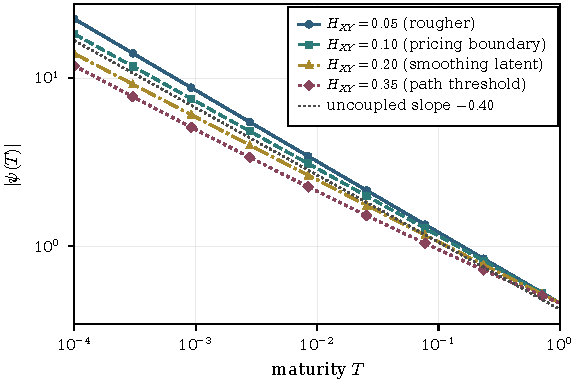
\includegraphics[width=0.78\textwidth]{figures/1-q-threshold-skew-scaling.pdf}
\caption{Bachelier ATM skew scaling $|\psi(T)|$ for several values of $H_{XY}$. The dominant short-maturity exponent is $\min(H_Y,H_{XY})-\frac12$. The dashed line is the uncoupled benchmark with slope $H_Y-\frac12=-0.40$.}
\label{fig:skew-scaling}
\end{figure}

\subsection[\texorpdfstring{Path-space threshold under \(\PP\)}{Path-space threshold under P}]{\texorpdfstring{Path-space threshold under \(\PP\)}{Path-space threshold under P}}\label{subsec:numerics_P}

The path-space calculation uses the discrete analogue of the relative covariance operator,
\[
\mathcal R_N = C_{Y,N}^{-1/2}\,C_{XY,N}\,C_{Y,N}^{-1/2},
\]
constructed from the covariance matrices of the discretised Volterra kernels on a grid of size $N$.
The continuum theory identifies the Hilbert--Schmidt condition
\[
\mathcal R_{Y,XY} \in \mathfrak S_2
\qquad\Longleftrightarrow\qquad
H_{XY}>H_Y+\frac14.
\]
In finite dimension, the corresponding diagnostic is \(\operatorname{tr}(\mathcal R_N^2)\).

Figure~\ref{fig:p-threshold} shows \(\operatorname{tr}(\mathcal R_N^2)\) as the grid size
increases, for the four representative values
\[
H_{XY}\in\{0.10,\,0.25,\,0.35,\,0.45\}.
\]
For $H_{XY}=0.10$ and $H_{XY}=0.25$, the quantity grows with $N$, consistent with the
non-Hilbert--Schmidt regime.  For $H_{XY}=0.35$, the critical threshold, the behaviour is
borderline over the resolved range.  For $H_{XY}=0.45$, the supercritical case, the growth is
weaker.  This is the finite-dimensional trace of the path-space threshold in the smoothing regime.

\begin{figure}[t]
\centering
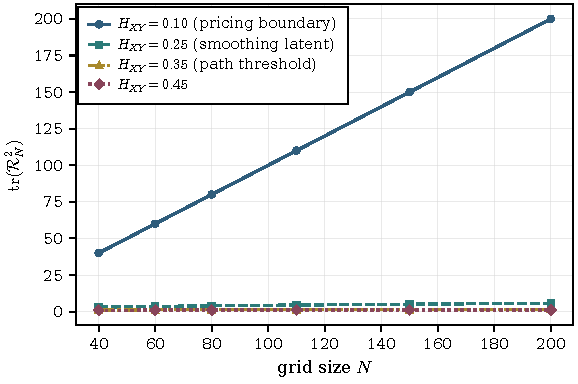
\includegraphics[width=0.78\textwidth]{figures/1-p-threshold-hilbert-schmidt-proxy.pdf}
\caption{Finite-dimensional proxy for the $\PP$-threshold. The quantity \(\operatorname{tr}(\mathcal R_N^2)\) grows with \(N\) in the non-Hilbert--Schmidt regime \(\delta<\frac14\), exhibits borderline behaviour at the critical threshold \(\delta=\frac14\), and shows weaker growth in the supercritical regime \(\delta>\frac14\).}
\label{fig:p-threshold}
\end{figure}

The finite-dimensional likelihood classifier compares the coupled and uncoupled Gaussian laws
(Figure~\ref{fig:classification}).  Discrimination is strongest in the non-smoothing benchmark
$H_{XY}=H_Y$.  Near and above the $\PP$-threshold, the finite-grid accuracy deteriorates over the
grid sizes considered.  This is consistent with the Feldman--H\'ajek dichotomy, since equivalence
of path laws precludes perfect separation on the limiting path experiment.

\begin{figure}[t]
\centering
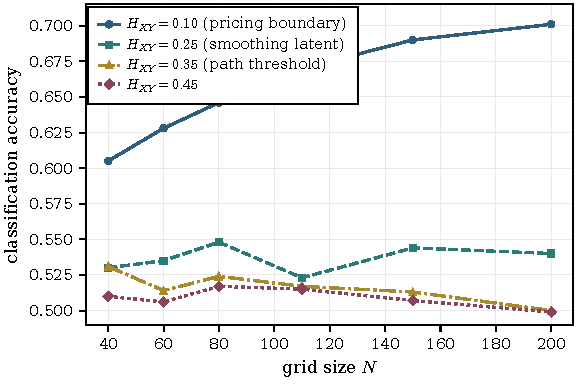
\includegraphics[width=0.78\textwidth]{figures/1-p-threshold-classification.pdf}
\caption{Likelihood-based classification accuracy for coupled versus uncoupled Gaussian path laws.}
\label{fig:classification}
\end{figure}

\subsection{Spectral asymptotics and latent energy}\label{subsec:numerics_spectral}

The theory predicts the eigenvalue asymptotics
\[
\lambda_n(\mathcal R_{Y,XY})\asymp n^{-2\delta},
\qquad
\delta=H_{XY}-H_Y>0,
\]
and cumulative spectral mass
\[
\mathcal E_{\mathrm{latent}}(N)\asymp N^{1-2\delta}.
\]

Figures~\ref{fig:spectrum-025} and \ref{fig:spectrum-035} display the ordered eigenvalues of the
finite relative covariance matrix on logarithmic axes for \(H_{XY}=0.25\) and \(H_{XY}=0.35\),
together with the theoretical reference slope.  In both cases the numerical spectra follow the
predicted power-law decay over the resolved range of modes.

\begin{figure}[t]
\centering
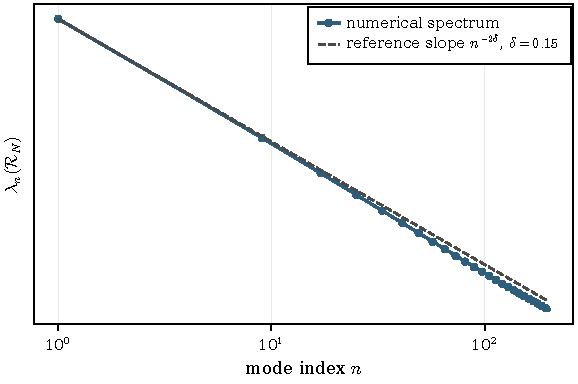
\includegraphics[width=0.78\textwidth]{figures/1-spectrum-decay-hxy-025.pdf}
\caption{Spectrum of \(\mathcal R_N\) for \(H_{XY}=0.25\) (\(\delta=0.15\)). The eigenvalues follow the predicted decay \(\lambda_n(\mathcal R_{Y,XY})\asymp n^{-2\delta}\).}
\label{fig:spectrum-025}
\end{figure}

\begin{figure}[t]
\centering
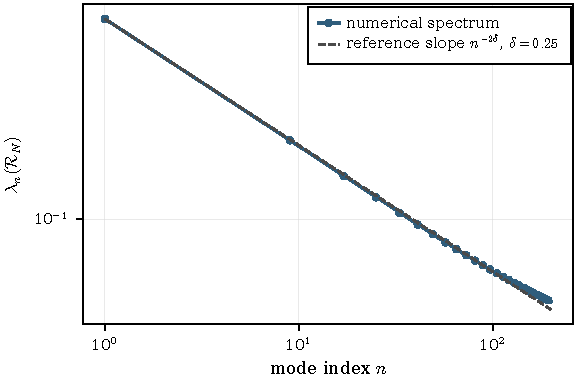
\includegraphics[width=0.78\textwidth]{figures/1-spectrum-decay-hxy-035.pdf}
\caption{Spectrum of \(\mathcal R_N\) for \(H_{XY}=0.35\) (\(\delta=0.25\)), corresponding to the critical \(\PP\)-threshold.}
\label{fig:spectrum-035}
\end{figure}

Figures~\ref{fig:latent-025} and \ref{fig:latent-035} show that the cumulative latent spectral
mass follows the predicted power law over the resolved range.  For $H_{XY}=0.25$, the growth is
approximately $N^{0.7}$.  For $H_{XY}=0.35$, the critical threshold, the growth is approximately
$N^{1/2}$.

\begin{figure}[t]
\centering
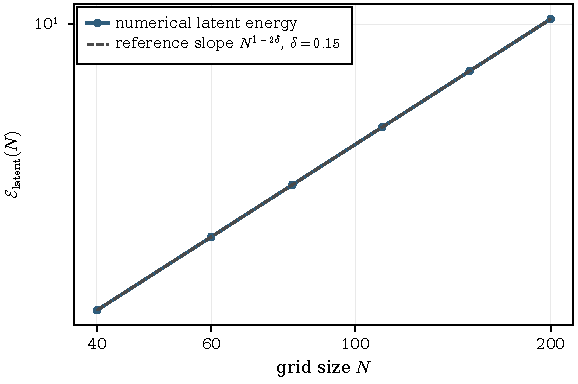
\includegraphics[width=0.78\textwidth]{figures/1-latent-energy-hxy-025.pdf}
\caption{Latent spectral energy for $H_{XY}=0.25$ ($\delta=0.15$). The growth agrees with the predicted scaling $N^{1-2\delta}$.}
\label{fig:latent-025}
\end{figure}

\begin{figure}[t]
\centering
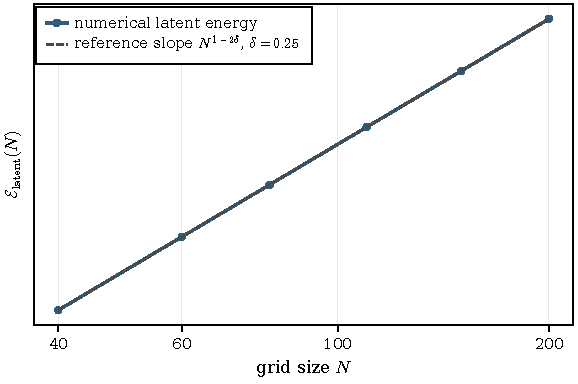
\includegraphics[width=0.78\textwidth]{figures/1-latent-energy-hxy-035.pdf}
\caption{Latent spectral energy for $H_{XY}=0.35$ ($\delta=0.25$), corresponding to the critical $\PP$-threshold. The energy grows as $N^{1/2}$.}
\label{fig:latent-035}
\end{figure}

\subsection{Summary}

The numerical diagnostics record the threshold separation:
\begin{enumerate}
\item On the \emph{pricing side}, the Bachelier ATM skew is dominated by the term with the smaller
Hurst exponent.  Once $H_{XY}>H_Y$, the cross-asset contribution is asymptotically invisible at
leading order.  The threshold is
\[
H_{XY}^{\Q}=H_Y.
\]

\item On the \emph{path-space side}, the relative covariance operator \(\mathcal R_{Y,XY}\) fails
to be Hilbert--Schmidt when \(\delta\le\frac14\), and the cumulative spectral mass grows according
to the predicted power law. The Feldman--H\'ajek threshold is
\[
H_{XY}^{\PP}=H_Y+\frac14.
\]

\item In the \emph{latent regime}
\[
H_Y < H_{XY} \le H_Y+\frac14,
\]
the pricing-side diagnostics show an invisible cross-asset component, while the path-space
diagnostics exhibit persistent spectral mass and nontrivial growth of the discrete
relative-covariance proxies.  The finite benchmark therefore separates pricing information from
statistical path information.
\end{enumerate}

%% ======================================================================
\section{Discussion}\label{sec:discussion}
%% ======================================================================

\subsection{Relation to existing multivariate rough volatility models}

The model~\eqref{eq:V}--\eqref{eq:logsig} is a bivariate Volterra stochastic volatility model
with heterogeneous Hurst exponents.  Dugo, Giorgio, and Pigato~\cite{DGP24} study a multivariate
fractional Ornstein--Uhlenbeck model with component-wise Hurst exponents and estimate asymmetric
cross-covariance spillovers by GMM on realised-volatility data.  The classification here has a
different object: Gaussian path-law distinguishability rather than spillover magnitude.

Bibinger, Yu, and Zhang~\cite{BYZ25} find empirically that multivariate fractional Brownian motion
forecasts outperform univariate ones when Hurst exponents diverge across assets.  That observation
is consistent with the threshold structure.  When $H_{XY}\ne H_Y$, the cross-asset component may
carry information at a roughness scale different from the idiosyncratic one.

\subsection{Relation to the correlation risk premium}

The divergence between $\Q$-measure and $\PP$-measure contagion thresholds is related to a
separate empirical boundary between implied and realised dependence.  Driessen, Maenhout, and
Vilkov~\cite{DMV09} show that option-implied correlation systematically exceeds realised
correlation, with the difference attributed to a large negative correlation risk premium.  Chen,
Wang \emph{et al.}~\cite{CWZL23} construct multiplex spillover networks from implied volatility,
realised volatility, and variance-risk-premium channels, and find non-redundant contagion
information across timescales.

The threshold comparison gives one formal route through which such $\Q$--$\PP$ divergence can
arise.  If the cross-Hurst exponent lies in the latent regime, the $\Q$-measure surface can be
insensitive at leading order to the contagion while $\PP$-measure path statistics are not.  This is
not a claim that the empirical correlation risk premium is caused by the latent regime.  The claim
is narrower: threshold separation is one channel through which $\Q$- and $\PP$-measure contagion
assessments can disagree.  Latent contagion then reflects a separation between statistical and
pricing observability rather than an additional risk factor.

\subsection{Limitations and caveats}

The model assumes log-normal volatility, Gaussian driving noise, and a time-invariant cross-exponent
\(H_{XY}\).  Empirical Hurst exponents may vary over time and may themselves be estimated with
error.  Cont and Das~\cite{CD24} show that microstructure noise can make standard volatility appear
rougher than it is, which complicates estimation of both \(H_Y\) and \(H_{XY}\).  The threshold
picture is a model statement; empirical use depends on exponent estimation.

The factor $\tfrac14$ in the path-detectability threshold is exact within the model.  It should not
be read with spurious precision in applications.  In finite samples, the boundary between the latent
and absorbed regimes is not sharp.  Detectability depends on sample size, sampling frequency, and
noise level.  The analysis also relies on Gaussian Volterra structure; non-Gaussian or jump-driven
extensions require different path-law tools.

%% ======================================================================
\section{Conclusion}\label{sec:conclusion}
%% ======================================================================

The bivariate rough Volterra experiment separates two observation levels for a directed
cross-asset volatility channel.  The pricing threshold
\[
H^{\Q}_{XY}=H_Y
\]
governs leading-order Bachelier skew visibility.  The path-space threshold
\[
H^{\PP}_{XY}=H_Y+\tfrac14
\]
governs equivalence versus singularity of the coupled and uncoupled Gaussian laws in the smoothing
regime.  The interval between them is the latent contagion regime: the directed channel is absent
from leading-order prices and still present in the physical path law.

Smooth non-degenerate modulation does not remove this separation.  Theorem~\ref{thm:T_asymp} shows
that, for $c>0$, the relative covariance operator has spectral order
\(\lambda_n(\mathcal R_{Y,XY})\asymp n^{-2\delta}\) with \(\delta=H_{XY}-H_Y>0\).  The fractional
singular-value order that governs the pure benchmark therefore continues to govern the modulated
Volterra model class used in practice.

The theorem remains a static threshold statement.  Observable screening, sequential revelation,
and feasible inference belong to separate experiments.  The Feldman--H\'ajek comparison proved here
is local to the smoothing regime \(H_{XY}>H_Y\), and finite samples replace the path-space dichotomy
by a sequence of statistical experiments.

Two residual questions remain.  The first is how far the smooth-modulation hypotheses can be
weakened without changing the threshold order.  The second is whether an analogue survives outside
Gaussian Volterra structure, where the Feldman--H\'ajek mechanism no longer decides path-law
comparison.  Pricing visibility and path-law detectability are different projections of the same
rough channel.

\bibliographystyle{unsrt}
\bibliography{references}

\end{document}
